% 회로도 부록: 보드마다 설명을 쓰고 그 뒤에 KiCad 회로도를 그대로 싣는다
% (시트의 PDF는 report/figures/make_schematic_figures.py로 생성).
\chapter{회로도}\label{app:schematics}

이 부록은 이 프로젝트가 만든 보드 다섯 장의 회로도다. 보드마다 먼저 무엇을 하는 보드인지, 시트가 어떻게
나뉘어 있는지, 전류가 어느 길로 흐르는지, 어떻게 확인했는지를 적고 그 뒤에 KiCad 회로도를 그대로 싣는다.
회로도는 쪽마다 한 시트이며 벡터 그림이므로 PDF에서 확대해 읽는다.

다섯 장에 공통인 것이 셋 있다.

\begin{itemize}
\item \textbf{회로도는 스크립트가 만든다.} 릴레이 130개를 손으로 그리면 선 하나가 틀려도 눈으로 찾을 수 없다.
그래서 회로를 ``단 $b$의 선 $i$의 릴레이는 어느 넷에 붙는가'' 같은 규칙으로 적고, 생성기(\code{gen\_*.py})가 그
규칙에서 KiCad 회로도를 쓴다. 생성물은 식별자를 고정해 두어 다시 만들어도 같은 파일이 나온다.
\item \textbf{확인은 넷리스트에서 한다.} 생성기가 맞는지를 생성기로 확인할 수는 없다. 검증 스크립트는 KiCad가
내보낸 넷리스트(어느 핀이 어느 넷에 붙어 있는가)만 읽고, 릴레이 접점과 다이오드를 스위치로 보아 회로를 풀어
소프트웨어 기준 모델과 견준다. 그다음 넷리스트를 일부러 한 곳씩 틀리게 바꾸어, 검증이 그것을 잡아내는지를
본다(음성 시험). 틀린 회로를 통과시키는 검증은 통과해도 뜻이 없기 때문이다.
\item \textbf{릴레이와 커넥터.} 릴레이는 모두 소형 신호 릴레이 G6S-2(접점 두 벌, 24~V 코일)이고 코일마다
역기전력 다이오드가 붙는다. 보드의 D-sub는 핀(수)이고 케이블의 양 끝이 소켓이며, 26선 커넥터는 1--26번이 선
A--Z다. 신호는 24~V 레벨이다. 이 규약은 저장소의 \code{docs/decisions/0003-interfaces.md}에서 정했고, 정한 뒤에
보드에서 고쳐야 할 곳은 각 절의 끝에 적었다.
\end{itemize}

배선(기판의 동선)은 아직 하지 않았다. 부품 배치는 부록~\ref{app:pcb}에 있다.

% ======================================================================
\section{릴레이 시프터 보드}\label{sch:shifter}

\paragraph{무엇을 하는가.} 릴레이식 스크램블러는 로터의 회전을 ``26선을 $a$칸 돌려 잇는 일''로 바꾸어 릴레이로
한다(\ref{sec:hw-relay}절). 이 보드는 그 시프터 한 쌍이다. 가는 길의 26선을 $+a$칸, 오는 길의 26선을 $-a$칸
옮긴다. 유닛 하나에 넉 장이 들어가고, 보드 사이에 로터 배선 카드와 반사판 카드가 끼인다. 릴레이 130개
(5단 $\times$ 26선), 다이오드 130개다. 능동 소자는 없다.

\paragraph{시트.} 루트 시트에 커넥터 다섯 개와 단 시트 다섯 장이 있다. 단 시트(\code{stage\_1}, \code{2}, \code{4},
\code{8}, \code{16})는 이동량만 다르고 모양이 같다: 릴레이 26개, 다이오드 26개, 단 표시등 하나. 모두 여섯 쪽이다.

\paragraph{왜 이렇게 이으면 시프트가 되는가.} 이동량 $s$인 단에서 선 $i$의 릴레이 하나를 본다
(그림~\ref{fig:sch-shifter-cell}). 접점 한 벌은 가는 길에 쓴다. 공통 단자가 입력의 $i$번 선이고, 놓여 있을 때 닫히는
쪽이 출력의 $i$번, 동작하면 닫히는 쪽이 출력의 $i+s$번이다. 26개가 함께 움직이므로 코일을 켜면 26선 전체가
$s$칸 옮겨지고 끄면 그대로 지나간다. 다섯 단(1, 2, 4, 8, 16칸)을 직렬로 이으면 켠 단의 이동량이 더해져 0에서
25까지의 모든 시프트가 된다. 제어값 $a$를 이진수로 적은 것이 곧 어느 단을 켤지다.

같은 릴레이의 다른 접점 한 벌은 오는 길에 쓰고 $i-s$번으로 잇는다. 코일이 하나이므로 가는 길이 $+a$이면
오는 길은 반드시 $-a$다. 에니그마의 로터를 지나갔다가 되돌아오는 전류가 같은 회전을 거꾸로 겪는다는 사실이
제어선 없이 배선으로 지켜진다. 단의 코일 26개는 제어선 하나(\code{CTRL})와 0~V 사이에 병렬이다.

\begin{figure}[ht]
\centering
\begin{tikzpicture}[x=1cm,y=1cm]
  \node[rcoil,minimum width=30mm,minimum height=30mm] (k) at (0,0) {};
  \node[font=\footnotesize] at (0,1.75) {릴레이 $K_{b,i}$ (접점 두 벌)};
  \node[font=\footnotesize,anchor=east] (oi) at (-2.2,0.5) {가는 길 입력 $i$};
  \node[font=\footnotesize,anchor=west] (oo) at (2.2,0.8) {가는 길 출력 $i$ (놓임)};
  \node[font=\footnotesize,anchor=west] (os) at (2.2,0.2) {가는 길 출력 $i+s$ (동작)};
  \node[font=\footnotesize,anchor=east] (ri) at (-2.2,-0.5) {오는 길 입력 $i$};
  \node[font=\footnotesize,anchor=west] (ro) at (2.2,-0.2) {오는 길 출력 $i$ (놓임)};
  \node[font=\footnotesize,anchor=west] (rs) at (2.2,-0.8) {오는 길 출력 $i-s$ (동작)};
  \draw (oi.east) -- (-0.6,0.5);
  \draw (ri.east) -- (-0.6,-0.5);
  \draw[cblue,line width=0.9pt] (-0.6,0.5) -- (0.6,0.8);
  \draw[cblue,line width=0.9pt] (-0.6,-0.5) -- (0.6,-0.2);
  \draw (0.6,0.8) -- (oo.west);
  \draw (0.6,0.2) -- (os.west);
  \draw (0.6,-0.2) -- (ro.west);
  \draw (0.6,-0.8) -- (rs.west);
  \foreach \p in {(-0.6,0.5),(-0.6,-0.5),(0.6,0.8),(0.6,0.2),(0.6,-0.2),(0.6,-0.8)} \fill \p circle (1.2pt);
  \node[font=\footnotesize,anchor=east] (c) at (-2.2,-1.2) {\code{CTRL}$_b$ (24 V)};
  \draw[->] (c.east) -- (-0.4,-1.2);
  \node[font=\scriptsize] at (0.3,-1.2) {코일 $\to$ 0 V};
\end{tikzpicture}
\caption{시프터 한 단의 릴레이 하나. 파란 선은 코일이 꺼져 있을 때 접점이 닿아 있는 쪽이다. 코일을 켜면 두 접점이
함께 아래로 넘어가 가는 길은 $+s$칸, 오는 길은 $-s$칸 옮겨진다.}
\label{fig:sch-shifter-cell}
\end{figure}

\paragraph{커넥터.} J1, J2가 가는 길과 오는 길의 입력, J3, J4가 출력이다(D-sub 37, 1--26번이 선 A--Z). J5는
제어(D-sub 9)로 1--5번이 단 1, 2, 4, 8, 16의 \code{CTRL}, 6--7번이 0~V다. 유닛에서 넷째 보드는 가는 길이
$-l$이어야 하므로 입력과 출력을 맞바꿔 잇는다. 회로가 대칭이어서 거꾸로 써도 시프터다.

\paragraph{전류.} 코일 하나는 24~V에서 5.8--8.3~mA(140--200~mW)다. 한 단을 켜면 26개와 표시등으로 약
0.16--0.22~A, 네 단을 켜는 최악(제어값 15나 23)에서 0.63--0.89~A가 든다. 제어값이 고르게 나오면 평균
8--11~W이고 유닛(넉 장)은 32--46~W다. 26선에 흐르는 시험 전류는 최대 약 0.2~A로 접점 정격 2~A에 견주어 작고,
전환은 시험 전압이 없는 동안에만 한다.

\paragraph{확인.} 전기 규칙 검사(ERC)는 위반 0건이다. 검증 스크립트는 넷리스트에서 제어값 0--25 각각에 대해
코일이 걸린 릴레이를 동작시키고 접점을 따라 연결을 추적한다. 26선 $\times$ 네 방향(가는 길, 오는 길, 거꾸로
끼운 가는 길과 오는 길)이 기준 모델 \code{relay.rs}의 $i+a$, $i-a$, $j-a$, $j+a$와 정확히 같고 그 밖의 연결이
하나도 없음을 확인한다. 26개 제어값이 모두 통과했다. 음성 시험은 다섯 가지다: 출력 커넥터의 두 핀을 바꾼
것 셋, 릴레이 하나의 두 접점을 바꾼 것, 제어선 둘을 바꾼 것. 다섯 모두 실패로 잡혔다.

\paragraph{고칠 곳.} 26선 커넥터의 27--29번은 지금 0~V에 이어져 있다. 스크램블러는 26선이 코일 전원과 떨어진
수동 소자여야 하므로 이 핀을 뗀다. 그대로 두면 코일의 복귀 전류가 메뉴 케이블로 나뉘어 흐른다.

\IfFileExists{figures/generated/sch_shifter-board.pdf}{%
  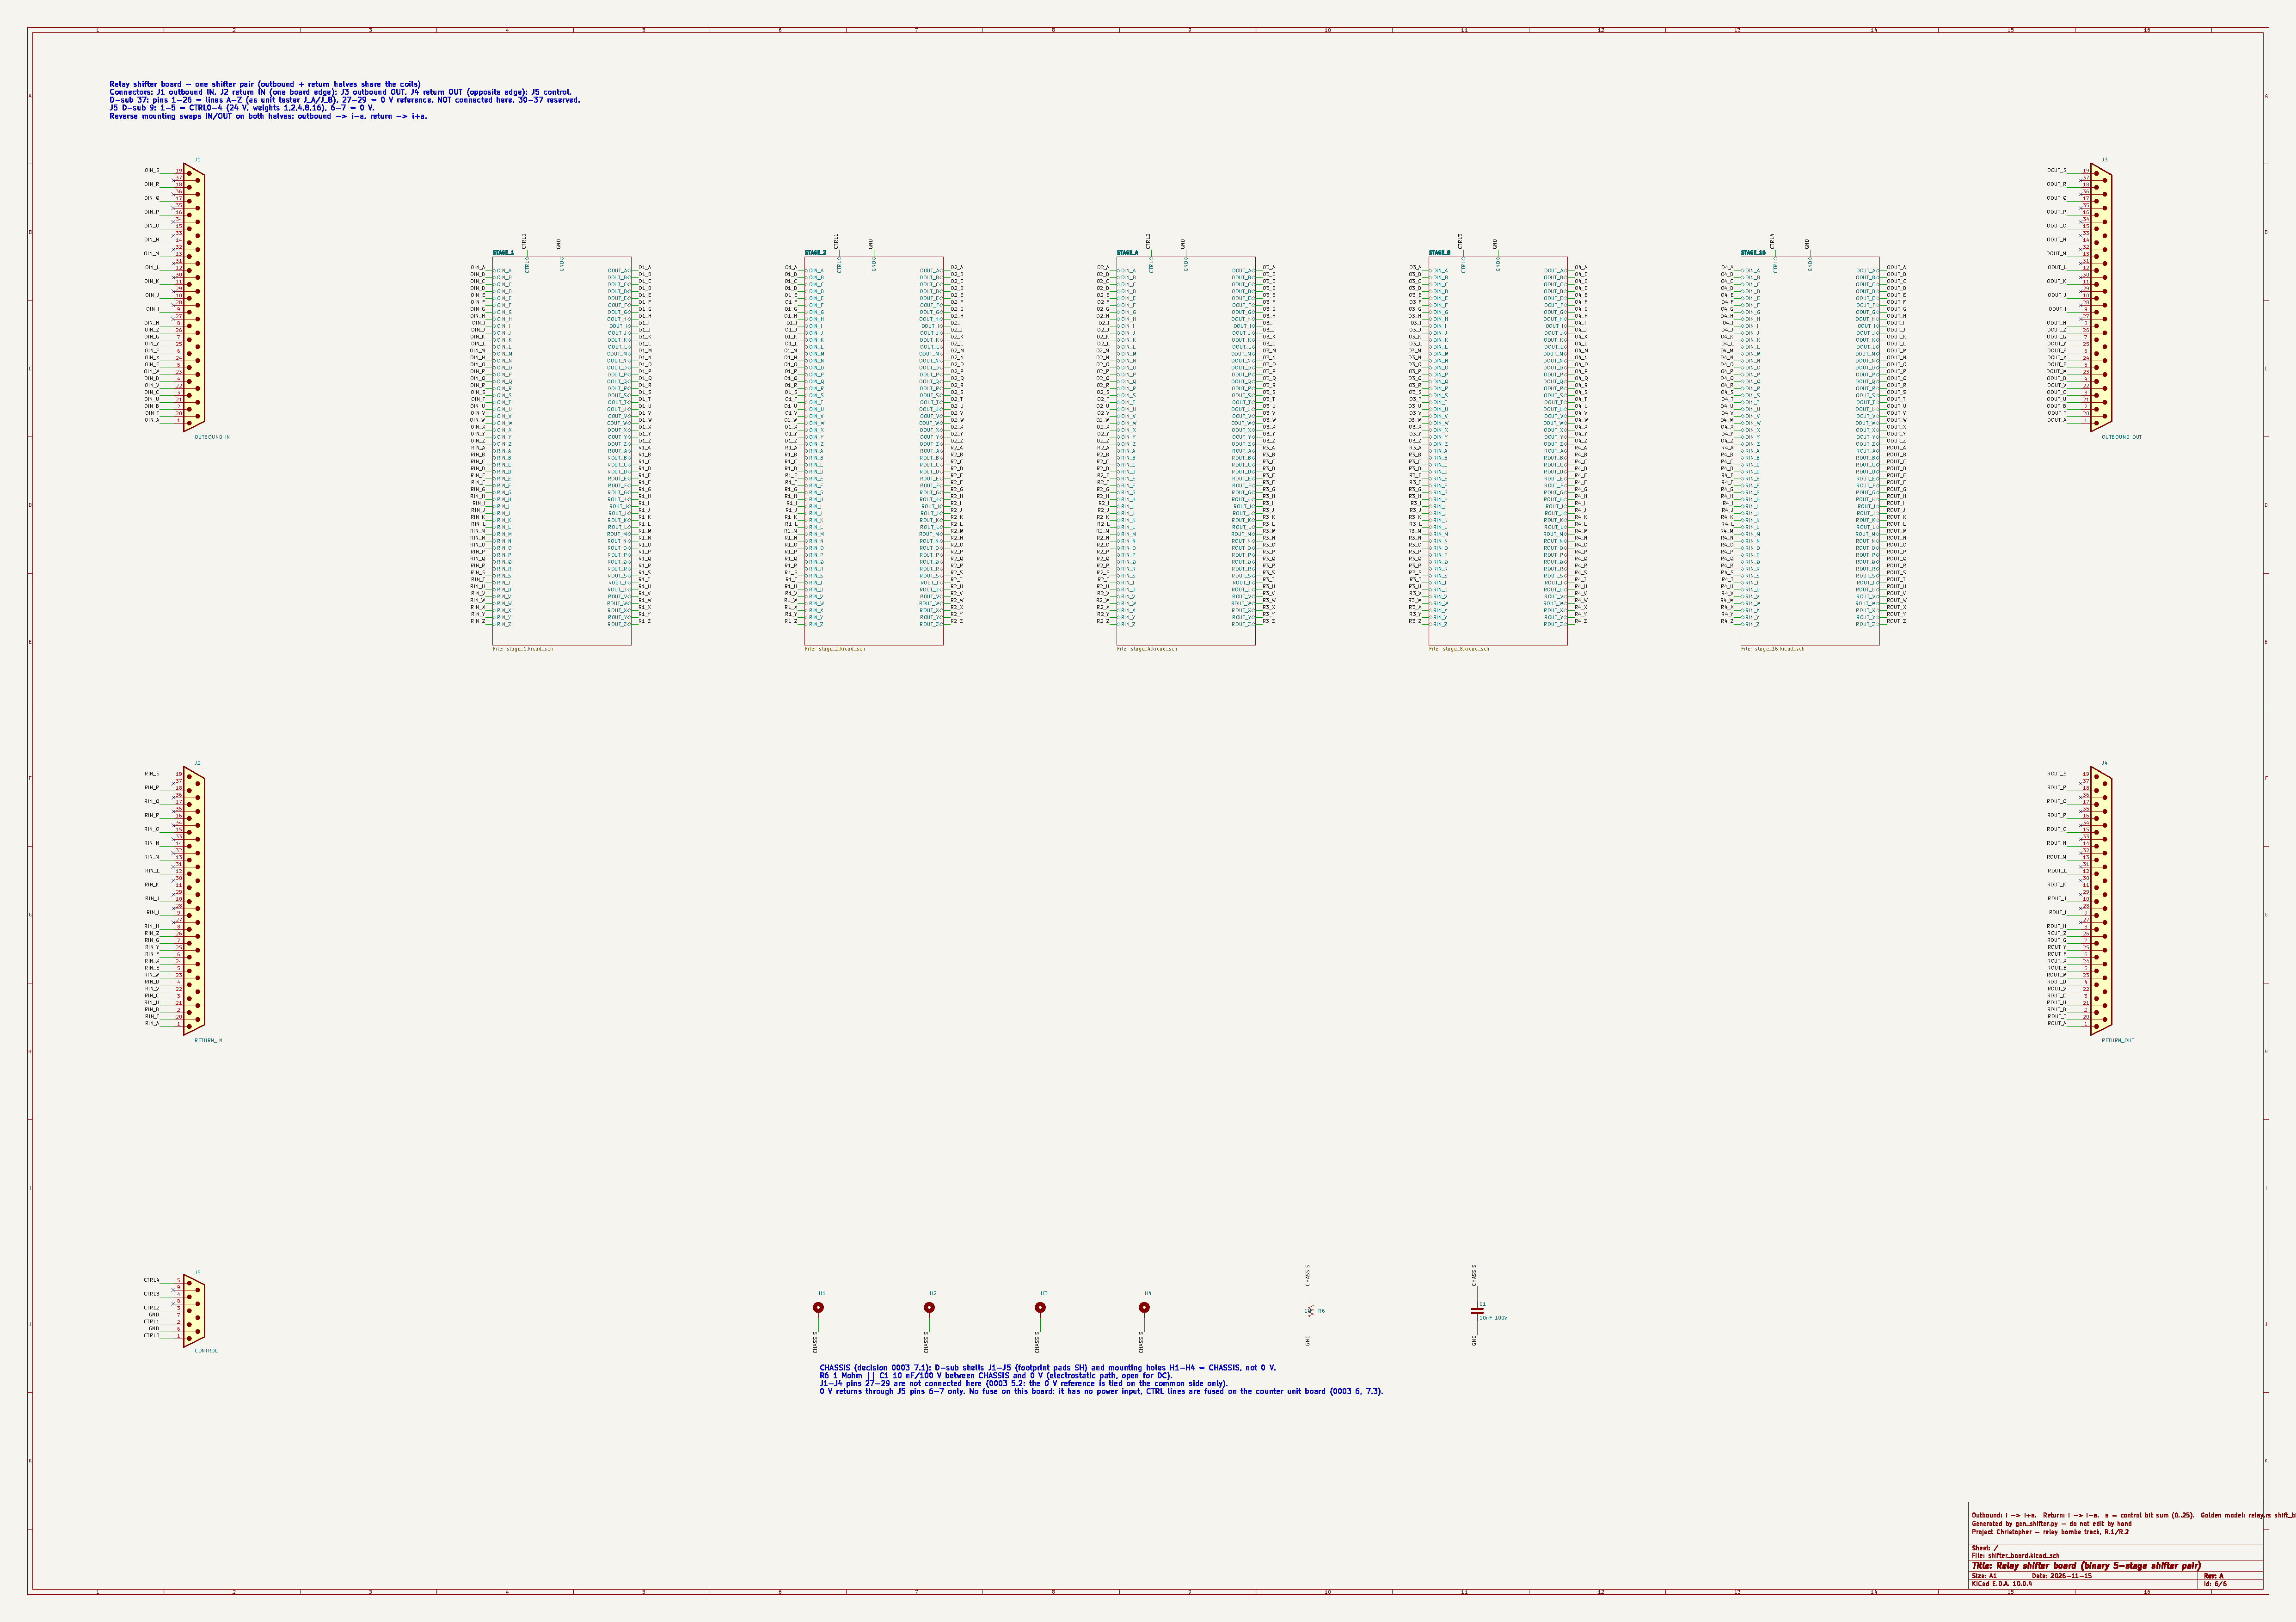
\includepdf[pages=-,pagecommand={\thispagestyle{plain}}]{figures/generated/sch_shifter-board.pdf}}{}

% ======================================================================
\section{릴레이 계수기 보드 (공통, 유닛)}\label{sch:counter-common}

\paragraph{무엇을 하는가.} 시프터의 제어값을 만드는 보드다. 드럼이 도는 대신 릴레이가 위치를 센다
(\ref{sec:hw-relay-counter}절). 세는 값은 다섯이다. $l$(빠른 자리), $m$(가운데 자리), 그리고 시프터에 바로 줄 수
있도록 미리 빼 둔 $a_3 = l - m$, $a_2$, $a_1$이다. 모든 자리가 같은 회로(릴레이 11개)이고 출력은 0--25의 5비트
이진수로, 시프터 보드의 \code{CTRL} 다섯 선을 그대로 구동한다. 보드는 두 장이다.

\begin{table}[ht]
\centering
\small
\begin{tabularx}{\linewidth}{l>{\raggedright\arraybackslash}Xrr}
\toprule
보드 & 내용 & 릴레이 & 다이오드 \\
\midrule
공통 & $l$, $m$, $a_3$ 세 자리와 자리 사이의 계수 규칙 전부. 뱅크에 한 장 & 33 & 196 \\
유닛 & $a_2$, $a_1$ 두 자리(다이얼로 정하는 시작값)와, 공통 보드의 $a_3$·$l$ 코드를 이 유닛의 시프터로 넘기는
중계 릴레이 10개. 유닛마다 한 장 & 32 & 138 \\
\bottomrule
\end{tabularx}
\end{table}

\paragraph{시트.} 공통 보드는 루트(커넥터와 자리 사이의 규칙 배선)와 자리 시트 석 장(\code{common\_pl},
\code{common\_pm}, \code{common\_a3})이다. 유닛 보드는 루트, 자리 시트 두 장(\code{unit\_a2}, \code{unit\_a1}), 중계
시트 한 장(\code{unit\_buf})이다. 자리 시트 다섯 장은 같은 회로다.

\paragraph{한 자리: 주종 쌍.} 비트마다 릴레이가 둘 있다. \emph{종(slave)}은 값을 갖고 그 접점이 출력을 낸다.
\emph{주(master)}는 평소에 종의 \emph{반대값}을 따라가고 있다. 한 자리를 1 올리는 일은 ``뒤집혀야 하는 비트의
종이 주의 값을 받는다''로 끝난다. 뒤집는 것이므로 새 값은 옛 값의 반대, 곧 주가 이미 갖고 있는 값이다.

왜 릴레이를 둘씩 쓰는가. 릴레이 하나로 뒤집으려 하면 그 릴레이의 접점이 자기 코일의 길을 바꾸므로, 펄스가
조금만 길어도 다시 뒤집힌다. 주가 다음 값을 미리 들고 있고 클럭 동안에는 변하지 않으면, 펄스의 길이와 무관하게
한 번만 넘어간다. 클럭은 두 상이다. 평상시(\code{NCK})에는 주가 종을 거울처럼 따라가고, 확정 펄스(\code{CK})
동안에는 주가 스스로를 붙잡고 종이 주의 값을 받는다. 두 상은 전환 접점 하나에서 나오므로 함께 켜지지 않는다.

\paragraph{올림 사슬.} 이진수에 1을 더하면 아래쪽의 1이 연달아 0이 되고 처음 만나는 0이 1이 된다. 곧 비트
$i$가 뒤집히는 조건은 ``아래 비트가 모두 1''이다. 이것을 주 릴레이의 접점을 직렬로 이은 사슬로 만든다.
증가 신호가 비트 0에서 들어가 주가 0인(= 종이 1인) 비트를 지나 위로 올라가고, 주가 1인 비트에서 멈춘다.
사슬이 닿은 비트가 뒤집히는 비트다. 주는 클럭 동안 변하지 않으므로 사슬은 접점만 지나갈 뿐 릴레이의 동작을
기다리지 않는다. 다섯 비트가 같은 순간에 넘어간다. 사슬이 닿지 않은 비트는 정지 레일로 제 값을 유지한다.
정지 레일은 ``사슬이 이 비트에 닿지 않았다''를 다이오드로 모아 만든 것이다.

\paragraph{25 다음은 0.} 5비트는 31까지 셀 수 있지만 자리는 26진이다. 값이 25(\code{11001})일 때에만 꺼지는
릴레이 하나(KW, 코일은 ``비트 0, 3, 4 가운데 하나라도 0''의 다이오드 합)가 비트 1과 2의 거울 길을 끊는다.
그러면 25에서 주는 \code{00110}이 아니라 \code{00000}이 된다. 주가 모두 0이면 사슬이 끝까지 올라가므로 다섯
비트가 모두 주의 값 0을 받고, 사슬의 끝이 곧 다음 자리로 가는 올림이다. 26이라는 중간값이 나타나지 않고,
따로 지우는 회로도 없다. 한 자리는 종 5, 주 5, KW 1로 릴레이 11개다.

\paragraph{자리 사이의 규칙.} $m$은 $l$이 25에서 0으로 넘어갈 때 오르고, $a_3 = l - m$은 매번 오르되 그때만
쉰다. $a_2$와 $a_1$도 같은 식의 규칙이다. 이 규칙은 앞 자리의 올림 레일과 ``25가 아님'' 레일을 다음 자리의
증가·정지 레일에 잇는 것으로 끝나며 모두 공통 보드에 있다. 유닛 보드에는 규칙이 없다. 레일 넷과 코드 열 선을
받아 세기만 하고, 시작값만 유닛마다 다이얼로 정한다($a_1 = k$, $a_2 = -k$. $k$는 그 유닛의 크립 오프셋).
규칙 신호가 모두 주의 값에서 나오므로 같은 클럭에서 종이 바뀌어도 흔들리지 않고, 자리 사이에 순서가 없다.

\paragraph{원위치.} 두 상을 모두 꺼서 릴레이를 전부 놓고, 적재 신호(\code{LOAD})로 종에 시작값을 넣은 다음,
평상시 상을 올리고 나서 적재 신호를 내린다. 순서가 바뀌어 틈이 생기면 넣은 값이 지워진다. 전원을 켠 직후의
임의 상태에서도 이 순서가 맞는 값을 만든다.

\paragraph{커넥터와 전류.} 공통 보드는 클럭(D-sub 9)과 유닛 버스(D-sub 25: 레일 넷, $l$과 $a_3$의 코드 열 선,
적재)를, 유닛 보드는 버스, 다이얼(D-sub 15), 시프터 넉 장으로 가는 제어 커넥터 넷(D-sub 9)을 갖는다. 한 자리는
늘 여섯쯤의 릴레이가 붙어 있어 1.1--1.5~W다. $a_1$과 $a_2$는 종의 접점이 시프터 한 단(약 0.2~A)을 바로 구동하고,
$a_3$과 $l$은 유닛마다 중계 릴레이를 거친다. 공통 보드의 접점 하나가 모든 유닛의 시프터를 떠맡지 않게 하려는
것이다.

\paragraph{확인.} ERC는 두 보드 모두 위반 0건이다. 검증 스크립트는 넷리스트만 읽어 접점 수준으로 풀고, 자기
유지가 있으므로 릴레이의 상태를 이어 가며 클럭을 넣는다. 기준은 \code{relay.rs}의 계수기를 옮긴 것이다.

\begin{itemize}
\item 자리 하나: 시작값 0--25 각각에서 증가와 정지를 섞은 60걸음(모두 1,560걸음)의 값과 올림.
\item 원위치: 크립 오프셋 26가지 전부, 릴레이의 처음 상태를 무작위로 두고. 순서를 바꾼 네 가지를 150번.
\item 전체 구동: 공통 한 장과 유닛 석 장을 한 시스템으로 묶어 17,576 클럭. 오프셋 0--25를 모두 거쳤다. 클럭마다
두 시점에서 모든 유닛의 제어값 넷과 내부 자리 다섯의 주·종 값을 기준과 견주었다. 불일치 0.
\item 경주: 바뀔 릴레이를 무작위 순서로 하나씩 넘기는 방식으로 17,576 클럭을 다시 돌렸다. 통과. 릴레이마다
빠르기가 달라도 결과가 같다는 뜻이다.
\item 음성 시험: 버스선, 접점, 다이오드의 방향, 다이얼의 비트, 커넥터 핀을 바꾼 14가지를 모두 잡았다.
\end{itemize}

이 시뮬레이션은 연결과 순서를 본다. 릴레이의 동작 시간과 코일 전압은 보지 않는다. 가장 깊은 길은 다이오드
넷을 지나므로 코일 전압이 1.2--1.6~V 깎인다. 그래서 보드의 전원 단자에서 23.0~V 이상을 요구한다.

\paragraph{고칠 곳.} 전원을 버스 커넥터로 받게 되어 있으나 유닛 하나가 최악 2.5--3.6~A를 쓰므로 보드마다 전원
단자를 따로 둔다. 뱅크의 위치(\code{POS})를 내보내는 커넥터가 없고, 느린 자리 $r$을 세는 자리도 없다(유닛의
$a_1$은 $r + k$다). 공통 보드에 자리 하나를 더한다.

\IfFileExists{figures/generated/sch_counter-common.pdf}{%
  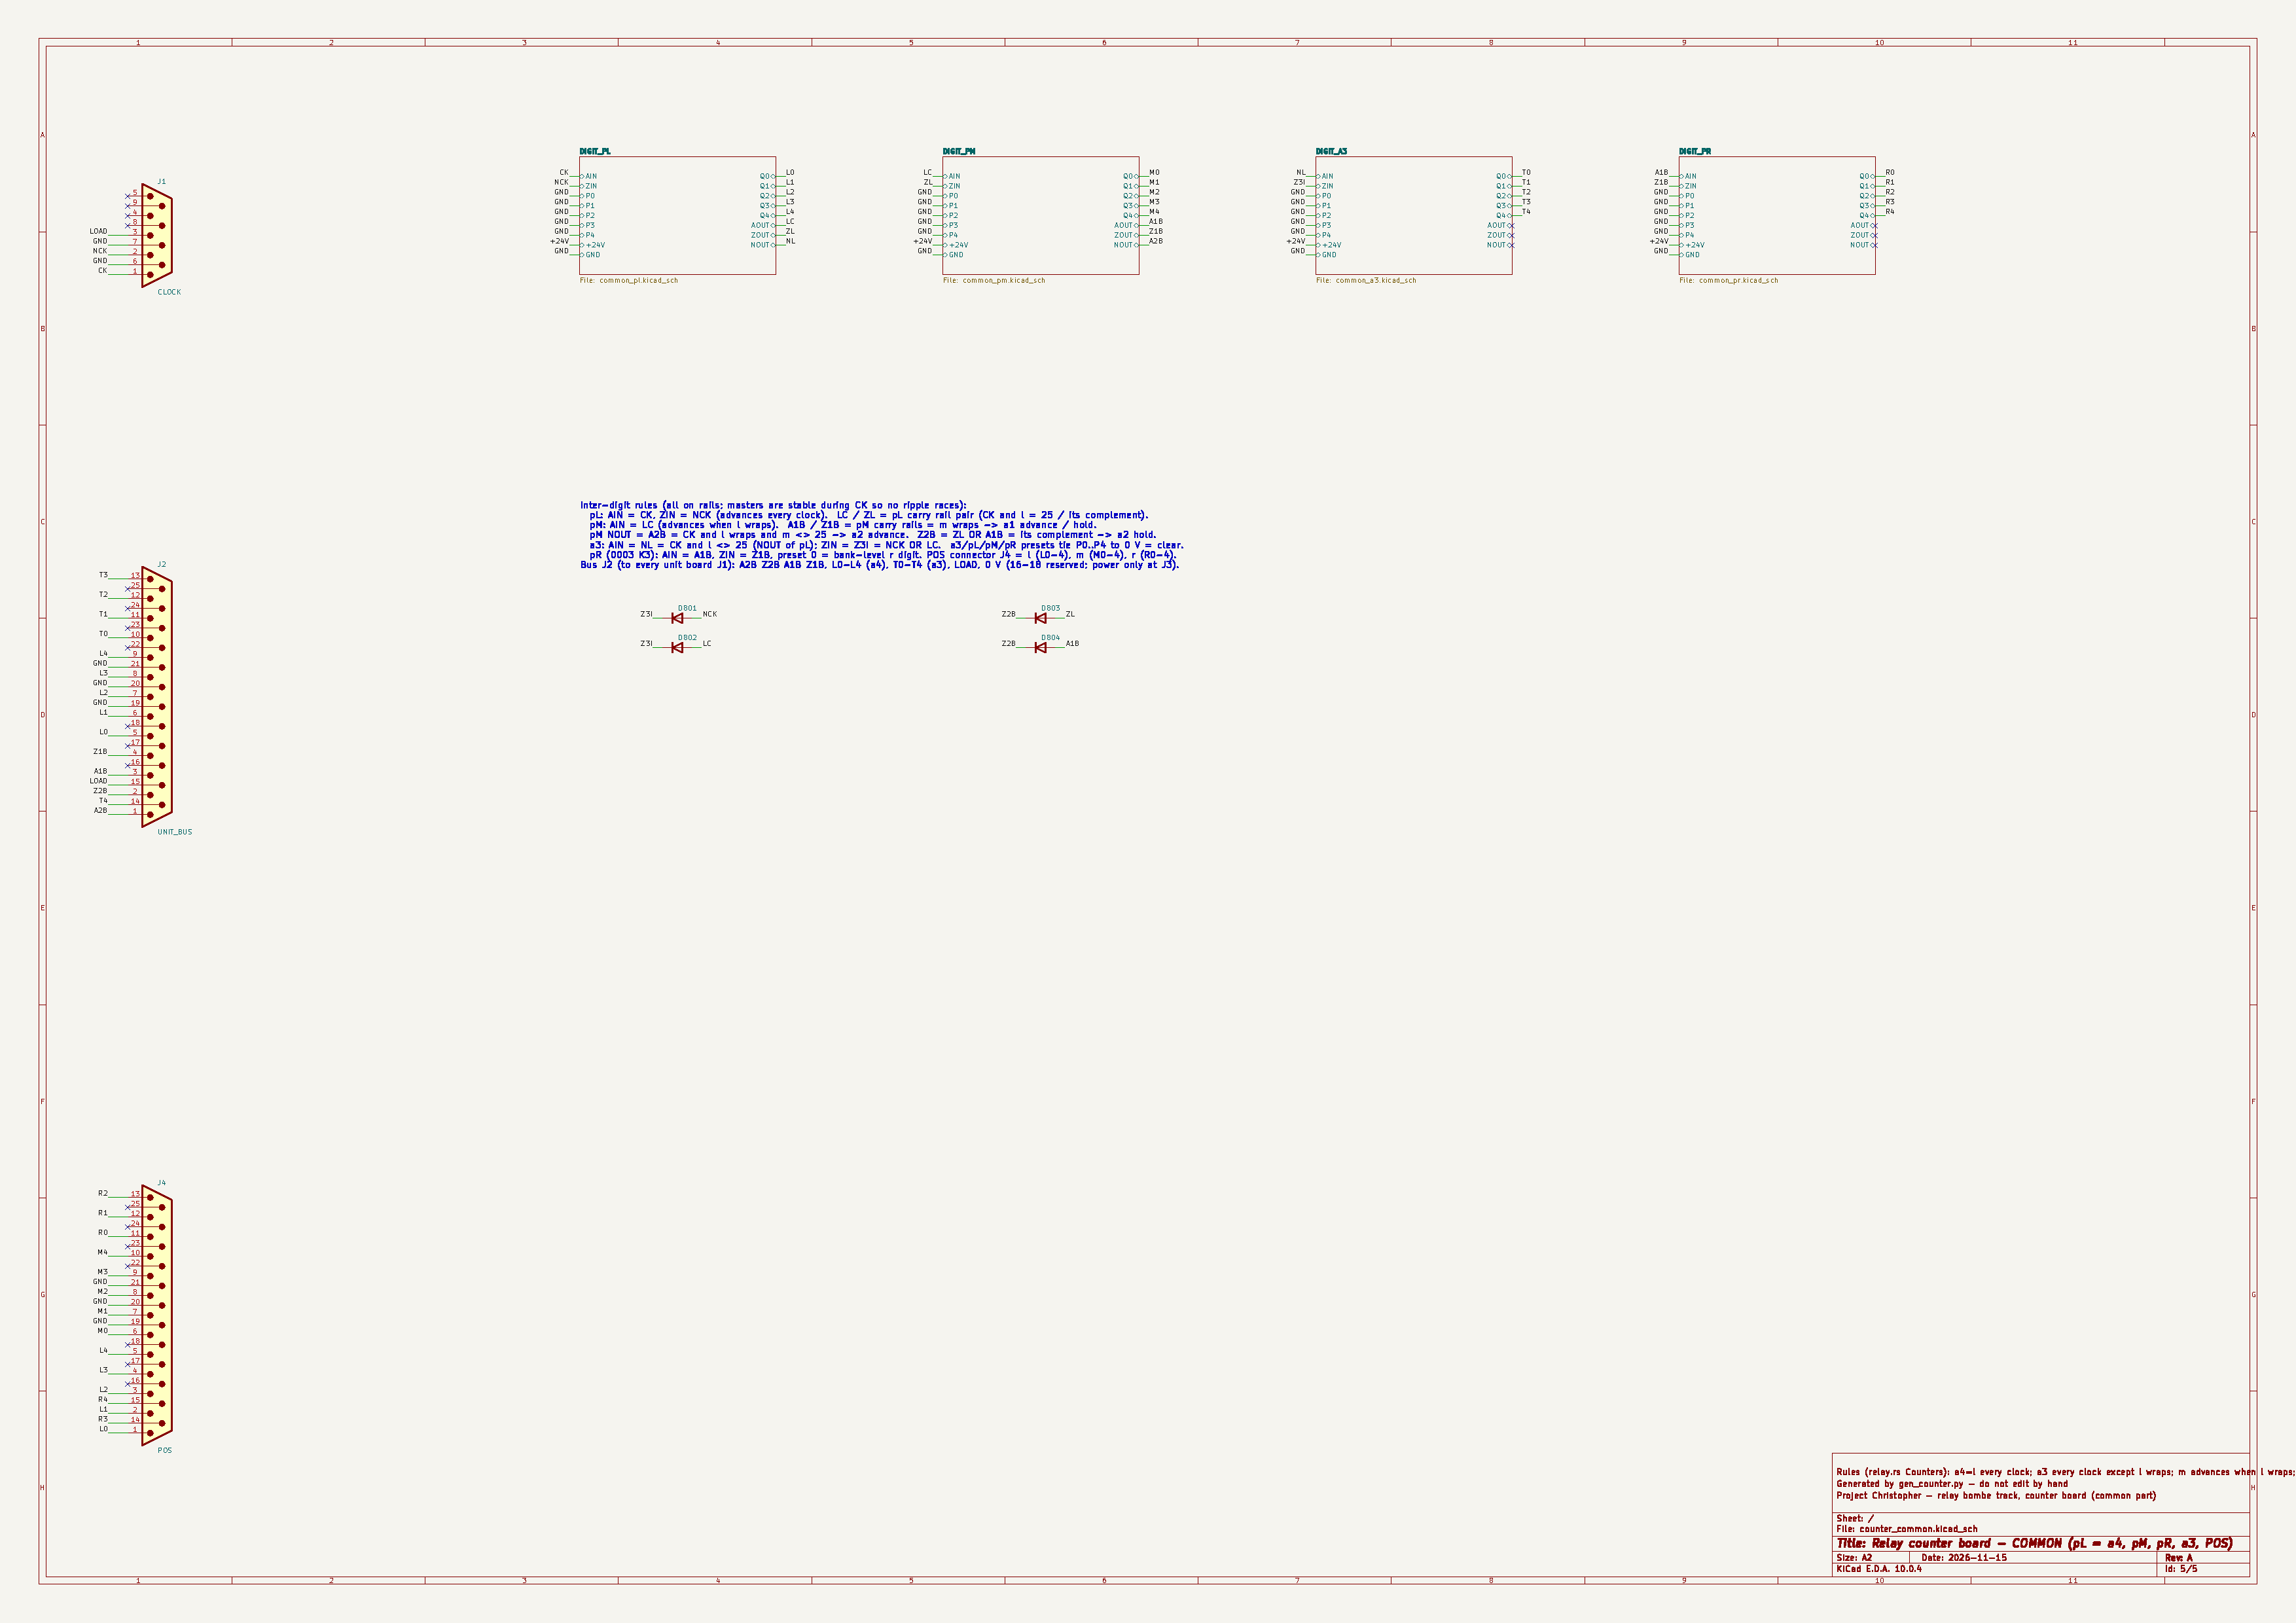
\includepdf[pages=-,pagecommand={\thispagestyle{plain}}]{figures/generated/sch_counter-common.pdf}}{}
\IfFileExists{figures/generated/sch_counter-unit.pdf}{%
  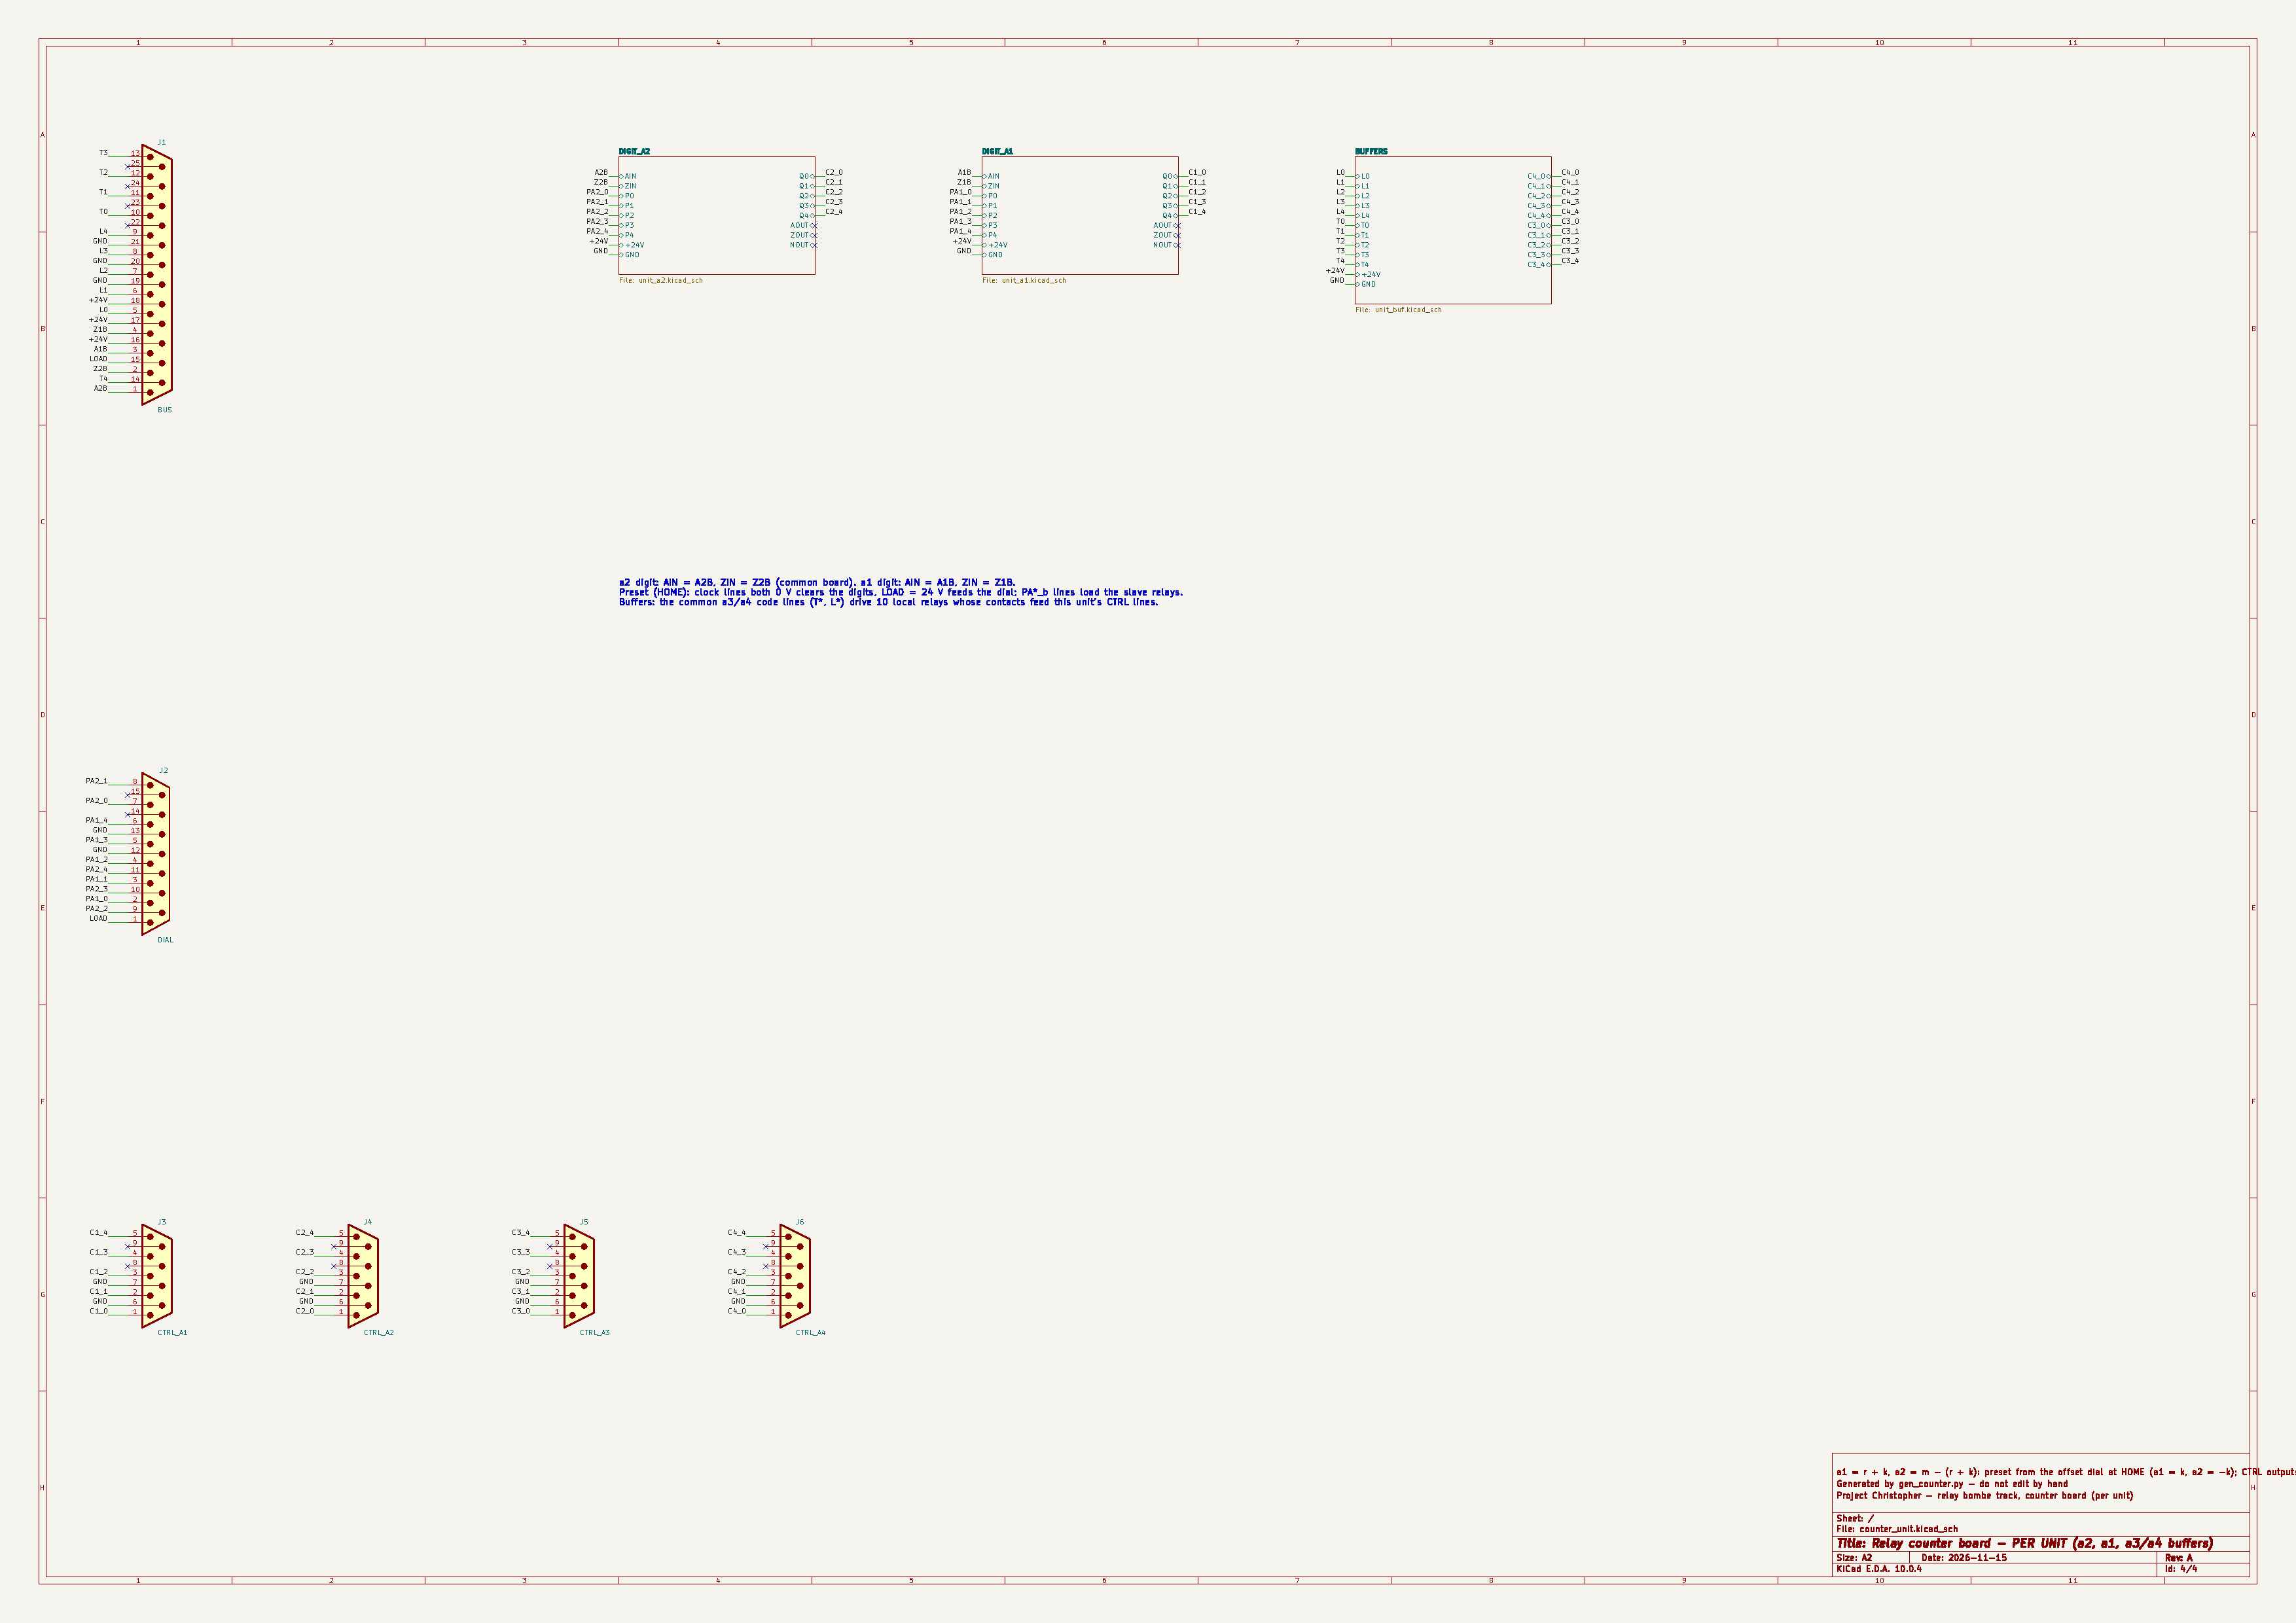
\includepdf[pages=-,pagecommand={\thispagestyle{plain}}]{figures/generated/sch_counter-unit.pdf}}{}

% ======================================================================
\section{테스트 레지스터 보드}\label{sch:test-register}

\paragraph{무엇을 하는가.} 공통부의 한가운데다. 입력 케이블의 26선을 받아 ``전부 통전되지는 않았는가''를
릴레이로 판정하고, 정지이면 뱅크를 세우고 그 순간의 26선을 붙들어 보여 준다. 원리와 그림은
\ref{sec:hw-register}절(그림~\ref{fig:hw-register})에 있다. 이 절은 그 회로가 보드에서 어떤 부품이 되었는지를
적는다. 신호 릴레이 34개, 표시를 구동하는 MOSFET 28개, 부품 258개다.

\paragraph{시트.} 두 장이다. \code{sense\_lanes}에는 같은 모양의 레인 26개가 있다. 레인 하나가 글자 하나다: 선에서
오는 차단 다이오드, 감지 릴레이(접점 한 벌은 자기 유지, 한 벌은 사슬), 코일 다이오드, 표시 구동(분압 저항 둘과
MOSFET), 보드 위의 표시등. 루트 시트에는 나머지가 있다: 타이밍 릴레이 셋, 통과 릴레이, 정지 릴레이 셋, 해제
릴레이, 정지 중에만 표시 쪽 0~V를 잇는 MOSFET, 커넥터, 전원의 퓨즈 둘.

\paragraph{한 위치에서 일어나는 일.} 그림~\ref{fig:hw-register}의 번호로 적는다.

\begin{enumerate}
\item \textbf{감지}(0--6~ms). \code{STROBE} 릴레이의 접점이 닫혀 시험 전압이 나간다. 통전된 선의 레인에서 전류가
다이오드를 지나 감지 릴레이를 붙이고, 붙은 릴레이는 유지 버스 $H$에서 스스로를 유지한다(그림의 (1)).
\item \textbf{정착}(6--12~ms). 26개가 모두 붙었으면 사슬이 이어져 통과 릴레이가 붙는다((3)).
\item \textbf{판정}(12--19~ms). \code{JUDGE} 릴레이의 접점이 닫힌다. 통과 릴레이가 놓여 있으면 그 b접점을 지나
정지 릴레이 셋이 붙어 자기 유지에 들어간다((4)). 정지 릴레이는 유지 버스를 우회해 감지 릴레이를 붙들고,
시험 전압을 끊고, \code{RUN}을 끊고, 표시 쪽 0~V를 이어 램프를 켠다.
\item \textbf{복귀}(21--33~ms). \code{CLEAR} 릴레이의 b접점이 열려 $H$가 끊기고 감지 릴레이와 통과 릴레이가
놓인다((2)). 정지 중이면 우회 때문에 아무것도 놓이지 않는다.
\end{enumerate}

\paragraph{보드로 옮기며 고친 네 곳.} 넷리스트를 릴레이의 동작·복귀 시간을 넣어 시뮬레이션하자 계산으로 정한
회로의 네 곳이 틀린 것으로 드러났다. 사슬을 $+24$~V가 아니라 $H$에서 먹일 것(통과 릴레이가 늦게 놓여 다음
위치의 정지를 놓친다), 통과 릴레이의 유지 접점에 직렬 다이오드를 넣을 것($H$가 거꾸로 살아난다), 정지 잠금과
정지 릴레이의 자기 유지를 $HSUP$에서 받을 것(해제 하나로 다 풀리게), 해제 릴레이를 둘 것(재출발 때 레지스터를
비운다). 이유는 \ref{sec:hw-register}절에 풀어 적었다.

\paragraph{왜 표시는 접점이 아니라 MOSFET인가.} 표시용 큰 릴레이 26개의 코일 전류는 합해 약 1~A다. 감지
릴레이의 접점으로 구동하면 이 전류가 유지 버스와 유지 접점을 지난다. 그래서 감지 릴레이의 코일 마디 전압을
분압해 MOSFET의 게이트에 주고, 표시 전류는 표시 커넥터의 $+24$~V(따로 2~A 퓨즈)에서 표시 릴레이와 MOSFET을
지나 0~V로 흐르게 했다. 판정의 길에는 전자 부품이 없다.

\paragraph{커넥터.} J1이 26선 입력, J2가 뱅크 제어(1번 \code{STROBE}, 2번 \code{RUN}, 3번 \code{STOPPED}, 34번
\code{JUDGE}, 35번 \code{CLEAR}, 36번 \code{STOP\_LATCH}), J3이 표시(1--26번 글자, 27번 정지 램프, 열린 드레인),
J4가 24~V 입력, J5가 시험 전압 선, J6이 앞면 패널(시작, 해제)이다.

\paragraph{전류.} 코일 하나에 약 8~mA이므로 26선이 모두 붙고 나머지 릴레이까지 더한 최악이 약 0.3~A, 정지 중의
보드 위 표시등이 0.17~A다. 논리 쪽 퓨즈는 유지 전류 1.1~A다.

\paragraph{확인.} ERC는 위반 0건이다. 검증 스크립트는 넷리스트에서 접점, 다이오드, MOSFET을 풀어 시간에 따라
사건을 진행시키고, 뱅크의 신호와 메뉴 배선망을 흉내 낸다. 배선망은 \code{STROBE} 동안에는 통전된 선들을 시험
선에 잇고 그 밖의 시간에는 엉뚱한 선들을 이어, 유지 전압이 배선망으로 새는지도 함께 본다.

\begin{itemize}
\item 438개의 위치 주기, 정지 176회. 26선이 전부 통전된 위치에서 거짓 정지 0.
\item 사례: 26선 전부, 25선 26가지, 1선 26가지, 0선, 무작위 부분집합 120, 정지·정지 중 주행·해제를 섞은 순서 12,
릴레이가 모두 가장 느리거나 가장 빠른 경우.
\item 폭이 비정상인 \code{STROBE}(2--8~ms)와 무작위 릴레이 시간 60번: 놓친 정지 0, 거짓 정지 6(안전한 쪽).
\item 릴레이가 가장 느릴 때의 최소 폭: \code{STROBE} 5~ms, \code{JUDGE} 5~ms, \code{CLEAR} 10~ms.
\item 음성 시험 18가지(다이오드의 방향, 접점의 종류, 각 릴레이의 기능, 신호와 선의 뒤바뀜)를 모두 잡았다.
\end{itemize}

접점의 튐과 코일 전압의 강하는 모델에 없다. 시제품에서 잰다.

\paragraph{고칠 곳.} 타이밍 릴레이의 코일은 빨리 놓이도록 다이오드와 제너로 클램프했는데, 코일이 커넥터의 핀에
바로 붙어 있어 신호가 꺼질 때 핀이 약 $-31$~V까지 내려간다. 핀과 코일 사이에 다이오드를 하나씩 넣어 이 전압이
뱅크로 나가지 않게 한다. 그 밖에 패널 단자에 Home 버튼과 비상 정지의 자리, 커넥터 껍데기의 섀시 접지, 전원의
역극성 보호를 더한다.

\IfFileExists{figures/generated/sch_test-register.pdf}{%
  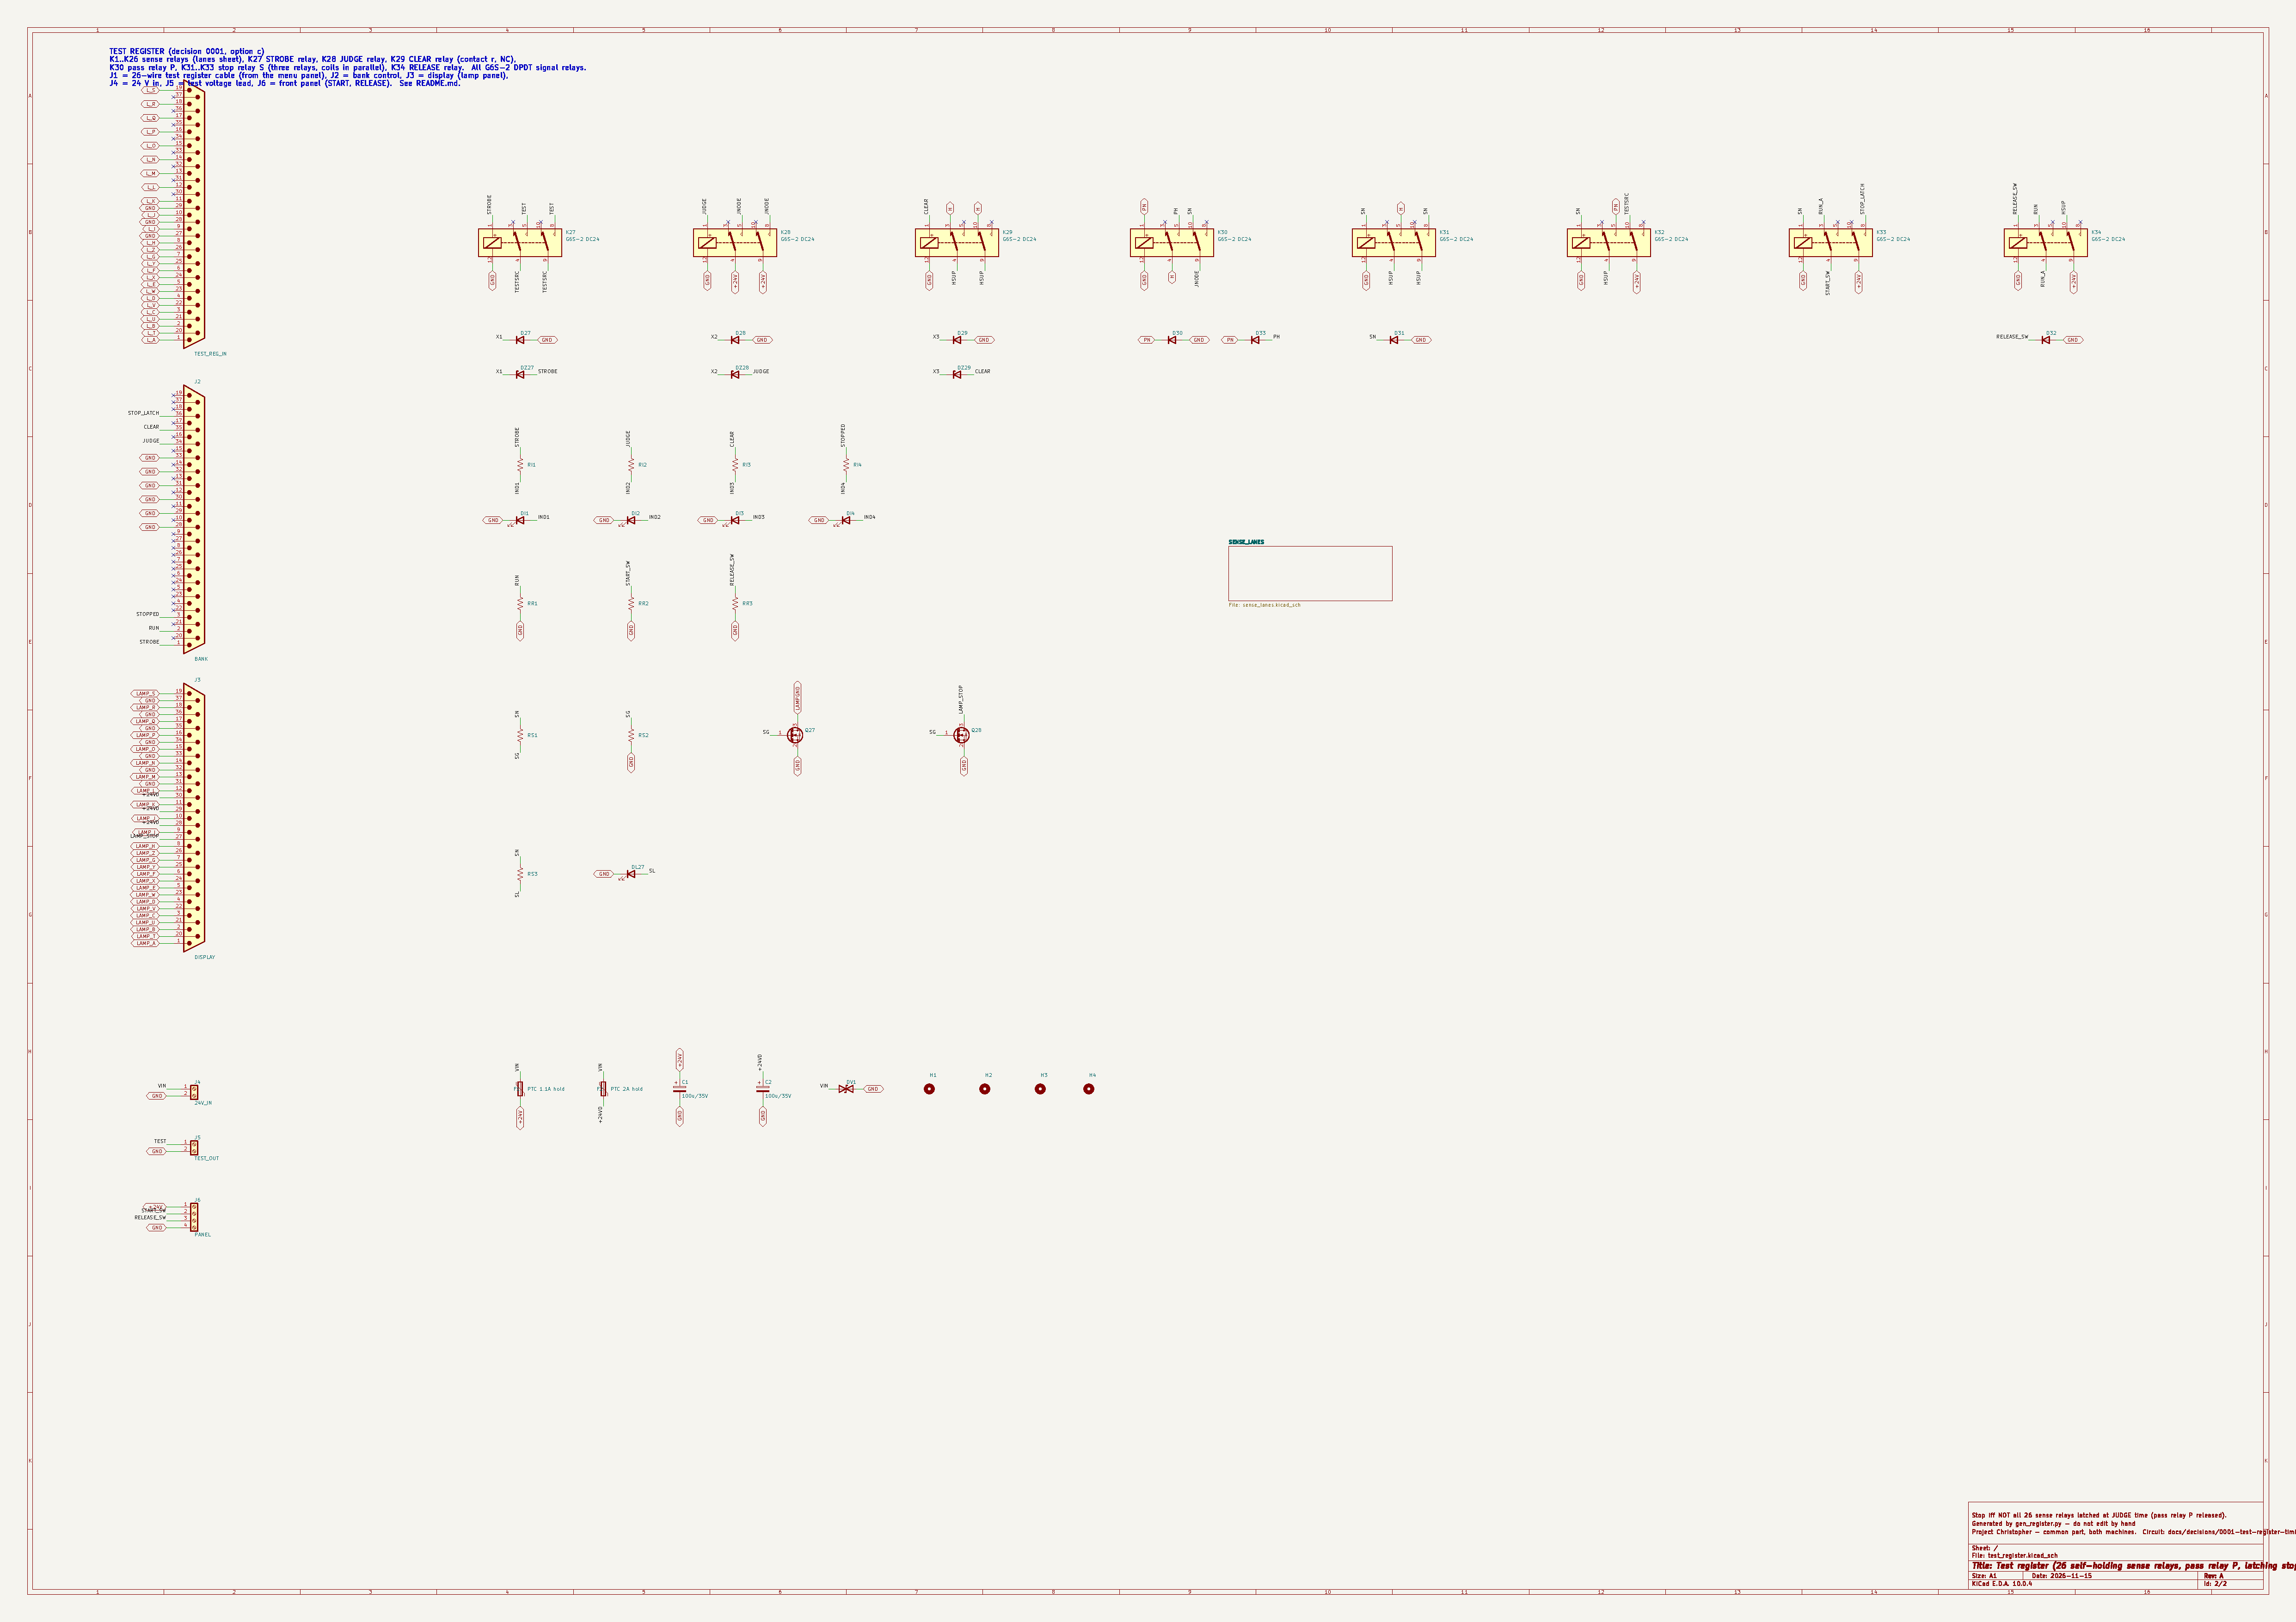
\includepdf[pages=-,pagecommand={\thispagestyle{plain}}]{figures/generated/sch_test-register.pdf}}{}

% ======================================================================
\section{스크램블러 단위 시험기}\label{sch:unit-tester}

\paragraph{무엇을 하는가.} 스크램블러 하나(또는 드럼 기판 한 장, 시프터 보드 한 장)를 꽂으면 26선과 26선
사이의 연결을 모두 읽어 소프트웨어 기준 모델과 견주는 장치다. 연결은 위치마다 $26 \times 26$개이고 위치가
17,576개이므로 손으로는 할 수 없다. 대상은 전원이 없는 수동 소자로 보고, 한쪽 26선을 A, 반대쪽 26선을 B라
부른다. 쓰는 순서는 \ref{sec:app-procedure}절에 있다.

\paragraph{한 노드의 구동과 감지.} 52선 하나하나가 같은 회로를 갖는다(그림~\ref{fig:sch-tester-node}). 구동 쪽은
고측 구동기 한 채널이 24~V를 1~k$\Omega$을 거쳐 선에 건다. 감지 쪽은 같은 선에서 2.2~k$\Omega$과 광커플러의
발광부를 거쳐 0~V로 간다. 한 선을 구동하면 그 선과 대상물 안에서 이어진 선의 광커플러가 켜진다. 한 번에 한
선씩 26번(또는 52번) 구동하고 그때마다 52선을 읽으면 연결의 표 전체가 나온다.

왜 24~V로 시험하는가. 접점 표면의 얇은 산화막은 낮은 전압과 작은 전류로는 뚫리지 않는다. 3.3~V로 읽으면
기계에서는 멀쩡히 통하는 접점을 끊어진 것으로 읽을 수 있다. 전시 기계와 같은 전압과 비슷한 전류(약 7~mA)로
읽어야 같은 답이 나온다. 1~k$\Omega$은 어떤 선이 0~V에 닿아도 전류를 24~mA로 묶는다.

\begin{figure}[ht]
\centering
\begin{tikzpicture}[x=1cm,y=1cm]
  \node[blkn] (pico) at (0,0) {Pico};
  \node[blkn] (iso) at (2.3,0.7) {절연기};
  \node[blkb] (sr) at (4.5,0.7) {74HC595};
  \node[blkb] (drv) at (6.9,0.7) {고측 구동기};
  \node[blk] (r1) at (9.2,0.7) {1 k$\Omega$};
  \node[circle,fill,inner sep=1.3pt] (n) at (10.8,0.7) {};
  \node[font=\footnotesize,anchor=west] at (11.0,0.7) {노드 $\to$ 커넥터의 선};
  \node[blk] (r2) at (9.2,-0.7) {2.2 k$\Omega$};
  \node[blko] (opt) at (6.9,-0.7) {광커플러};
  \node[blkb] (si) at (4.5,-0.7) {74HC165};
  \draw[->] (pico) |- (iso);
  \draw[->] (iso) -- (sr);
  \draw[->] (sr) -- (drv);
  \draw[->] (drv) -- (r1);
  \draw (r1) -- (n);
  \draw[->] (n) |- (r2);
  \draw[->] (r2) -- (opt);
  \draw[->] (opt) -- (si);
  \draw[->] (si) -| (pico);
  \draw[dashed,cred] (1.2,-1.5) -- (1.2,1.5);
  \draw[dashed,cred] (1.2,-0.05) -- (5.8,-0.05) -- (5.8,-1.5);
  \node[note,text=cred] at (0,1.3) {USB 쪽 (3.3 V)};
  \node[note,text=cred] at (8.0,1.5) {현장 쪽 (24 V)};
\end{tikzpicture}
\caption{단위 시험기의 한 노드. 위가 구동, 아래가 감지다. 점선이 절연 장벽이다. 구동은 디지털 절연기에서, 감지는
광커플러에서 장벽을 건넌다. 같은 회로가 52개 있다.}
\label{fig:sch-tester-node}
\end{figure}

\paragraph{절연.} 보드는 두 영역이다. 현장 쪽(24~V 어댑터: 구동기, 광커플러의 발광부, 구동용 시프트 레지스터)과
USB 쪽(Pico, 감지용 시프트 레지스터)이다. 현장 쪽의 0~V는 기계의 프레임과 모터 전원으로 이어질 수 있으므로
PC와 직접 닿으면 안 된다. 두 영역을 건너는 부품은 디지털 절연기 둘, \code{STROBE}용 고속 광커플러 하나, 감지
광커플러 열아홉뿐이다. 넷리스트 검사가 ``두 영역의 핀이 한 넷에 섞이지 않는다, 수동 소자가 두 영역을 잇지
않는다''를 확인한다(현장 쪽 넷 313개, USB 쪽 132개, 섞인 넷 0).

\paragraph{시트.} 루트와 하위 시트 14장이다. \code{power}(24~V 입력, 퓨즈, 5~V 강압), \code{mcu}(Pico),
\code{isolation}(절연기 둘과 \code{STROBE} 광커플러), \code{shift\_out}(74HC595 일곱 개), \code{shift\_in}(74HC165 열
개), \code{frontend\_g0}--\code{g6}(노드 여덟 개씩: 구동기 하나, 1~k$\Omega$, 2.2~k$\Omega$, 4채널 광커플러 둘),
\code{aux\_sense}(위치 15선, 뱅크의 상태 신호, 안전 사슬, \code{JUDGE}·\code{CLEAR}), \code{connectors}(D-sub 37 세 개와
저항 측정용 헤더).

\paragraph{뱅크와의 연결.} 세 번째 커넥터는 뱅크 제어 커넥터다. 시험기는 여기서 공통부의 자리에 선다.
\code{RUN}과 \code{HOME}을 내고, \code{STROBE}, 위치, 상태 신호를 읽는다. 대상이 스스로 돌아가는 동안
\code{STROBE}마다 한 번씩 읽으면 위치를 따라가며 시험할 수 있다. 구동기의 입력은 풀다운되어 있고 출력 허가는
풀업이어서, 부팅 중이거나 USB가 빠지면 모든 구동이 꺼진다.

\paragraph{확인.} ERC는 위반 0건이다(루트와 14장). 넷리스트 검사는 1,924가지를 확인했고 실패가 없다. 52노드
각각에서 시프트 레지스터의 비트 $\to$ 구동기 채널 $\to$ 1~k$\Omega$ $\to$ 노드 $\to$ 커넥터의 핀, 같은 노드에서
2.2~k$\Omega$ $\to$ 광커플러 $\to$ 시프트 레지스터의 같은 번호 비트로 이어지는지를 본다. 펌웨어의 핀 지도는 소스에서
읽어 넷리스트와 견준다. 넷 이름 두 쌍을 바꾼 넷리스트는 실패로 잡혔다. 펌웨어와 호스트 프로그램은 가상의
대상물(52노드의 도체 그래프에 결함을 넣은 것)로 시험했다. 실물로는 아직 시험하지 않았다.

\paragraph{고칠 곳.} 커넥터가 소켓이다. 다른 보드와 같은 케이블을 쓰도록 핀으로 바꾼다. \code{RUN}과
\code{HOME} 출력의 직렬 1~k$\Omega$은 뱅크의 입력이 릴레이 코일이면 전압이 모자라므로 자동 복귀 퓨즈로 바꾼다.
안전 사슬은 뱅크가 전원을 주는 고리로 바꾸고, \code{STOP\_LATCH}를 읽는 입력을 더한다.

\IfFileExists{figures/generated/sch_unit-tester.pdf}{%
  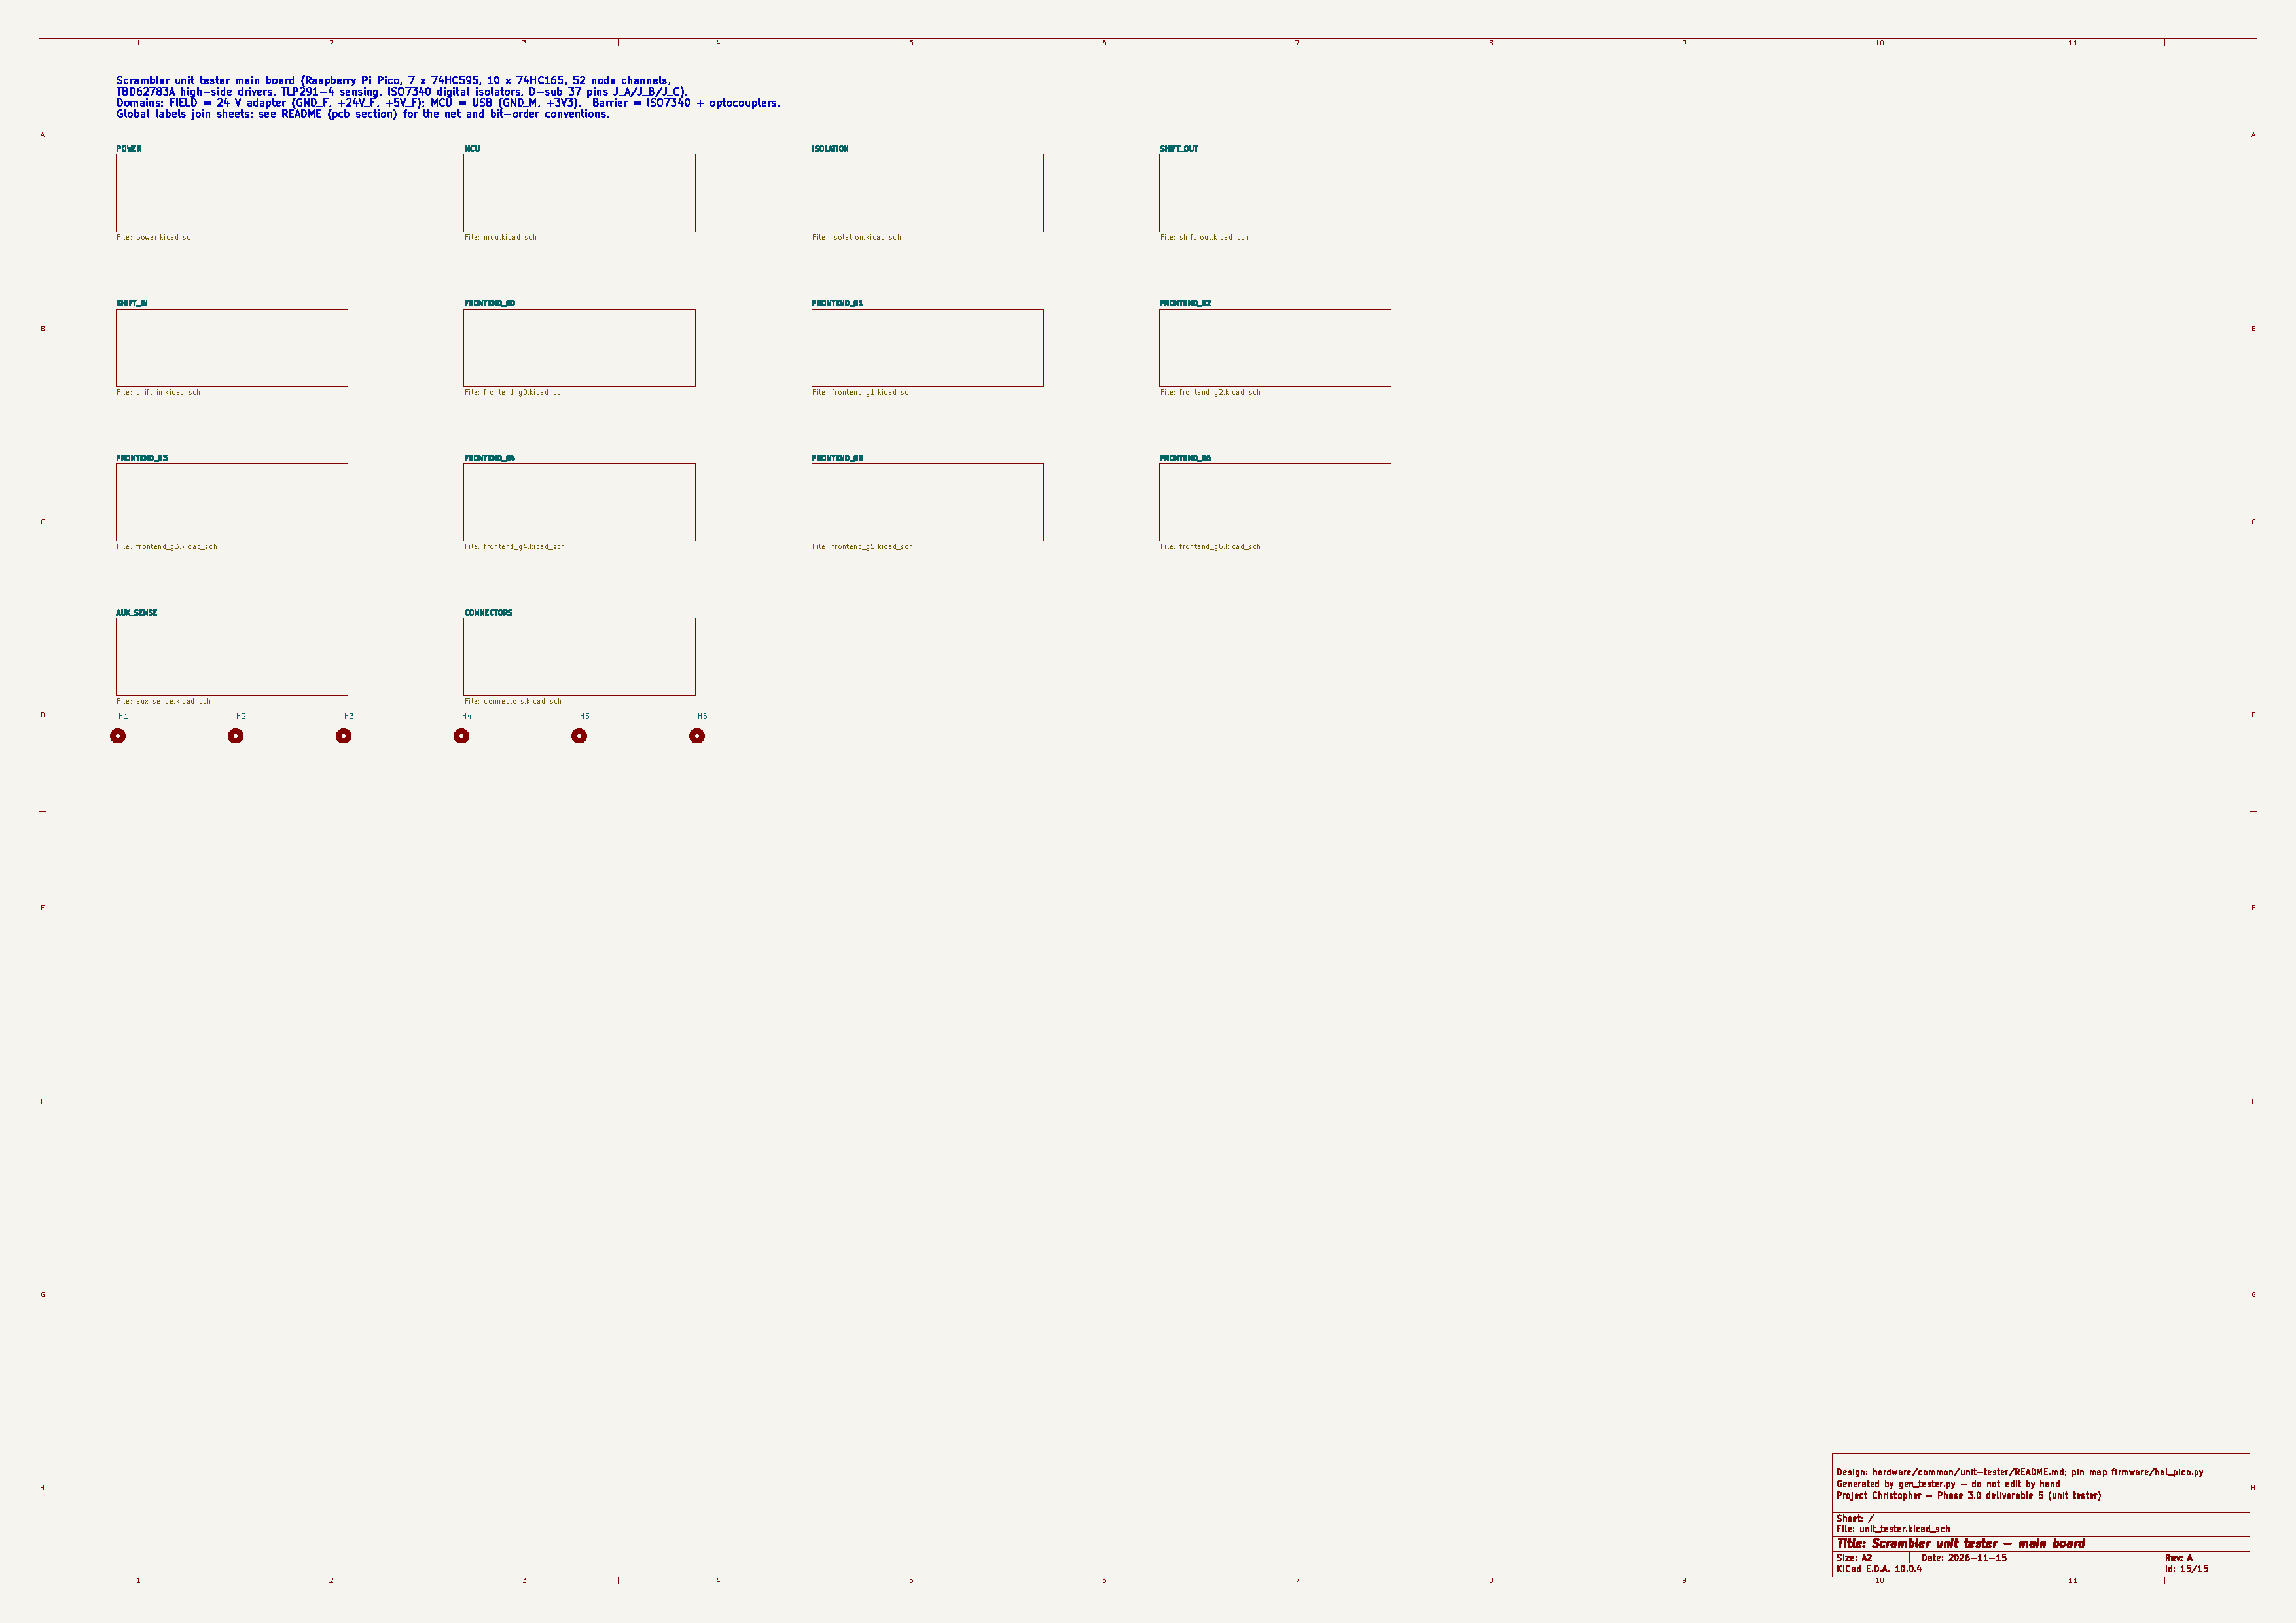
\includepdf[pages=-,pagecommand={\thispagestyle{plain}}]{figures/generated/sch_unit-tester.pdf}}{}

\section{기어식 접점 보드와 열 배선}\label{sch:contact-board}
드럼 한 자리마다 한 장인 접점 보드(Omniball 7845 접점 104개, 반지름 22/29/36/43\,mm의 네 링), 열의 입출력 단자,
반사판 배선 카드(B, C)다. 세 자리와 단자, 반사판 카드가 1:1 리본 여덟 가닥으로 이어져 한 열이 스크램블러 하나가
된다. \code{hardware/gear/contact-board/verify\_column.py}가 보드 파일에서 접점의 링과 위치를 읽어 열 전체를
조립하고, 로터 I--V의 60개 순서 × 17,576 위치 모두(1,054,560가지)에서 입력→출력 연결이 에니그마 스크램블러와
같음을 확인했다. 부정 시험(거울상 보드, 리본 핀 뒤바꿈, 잘못된 반사판 카드, 잘못된 링 등)은 모두 잡힌다.
\IfFileExists{figures/generated/sch_contact-board.pdf}{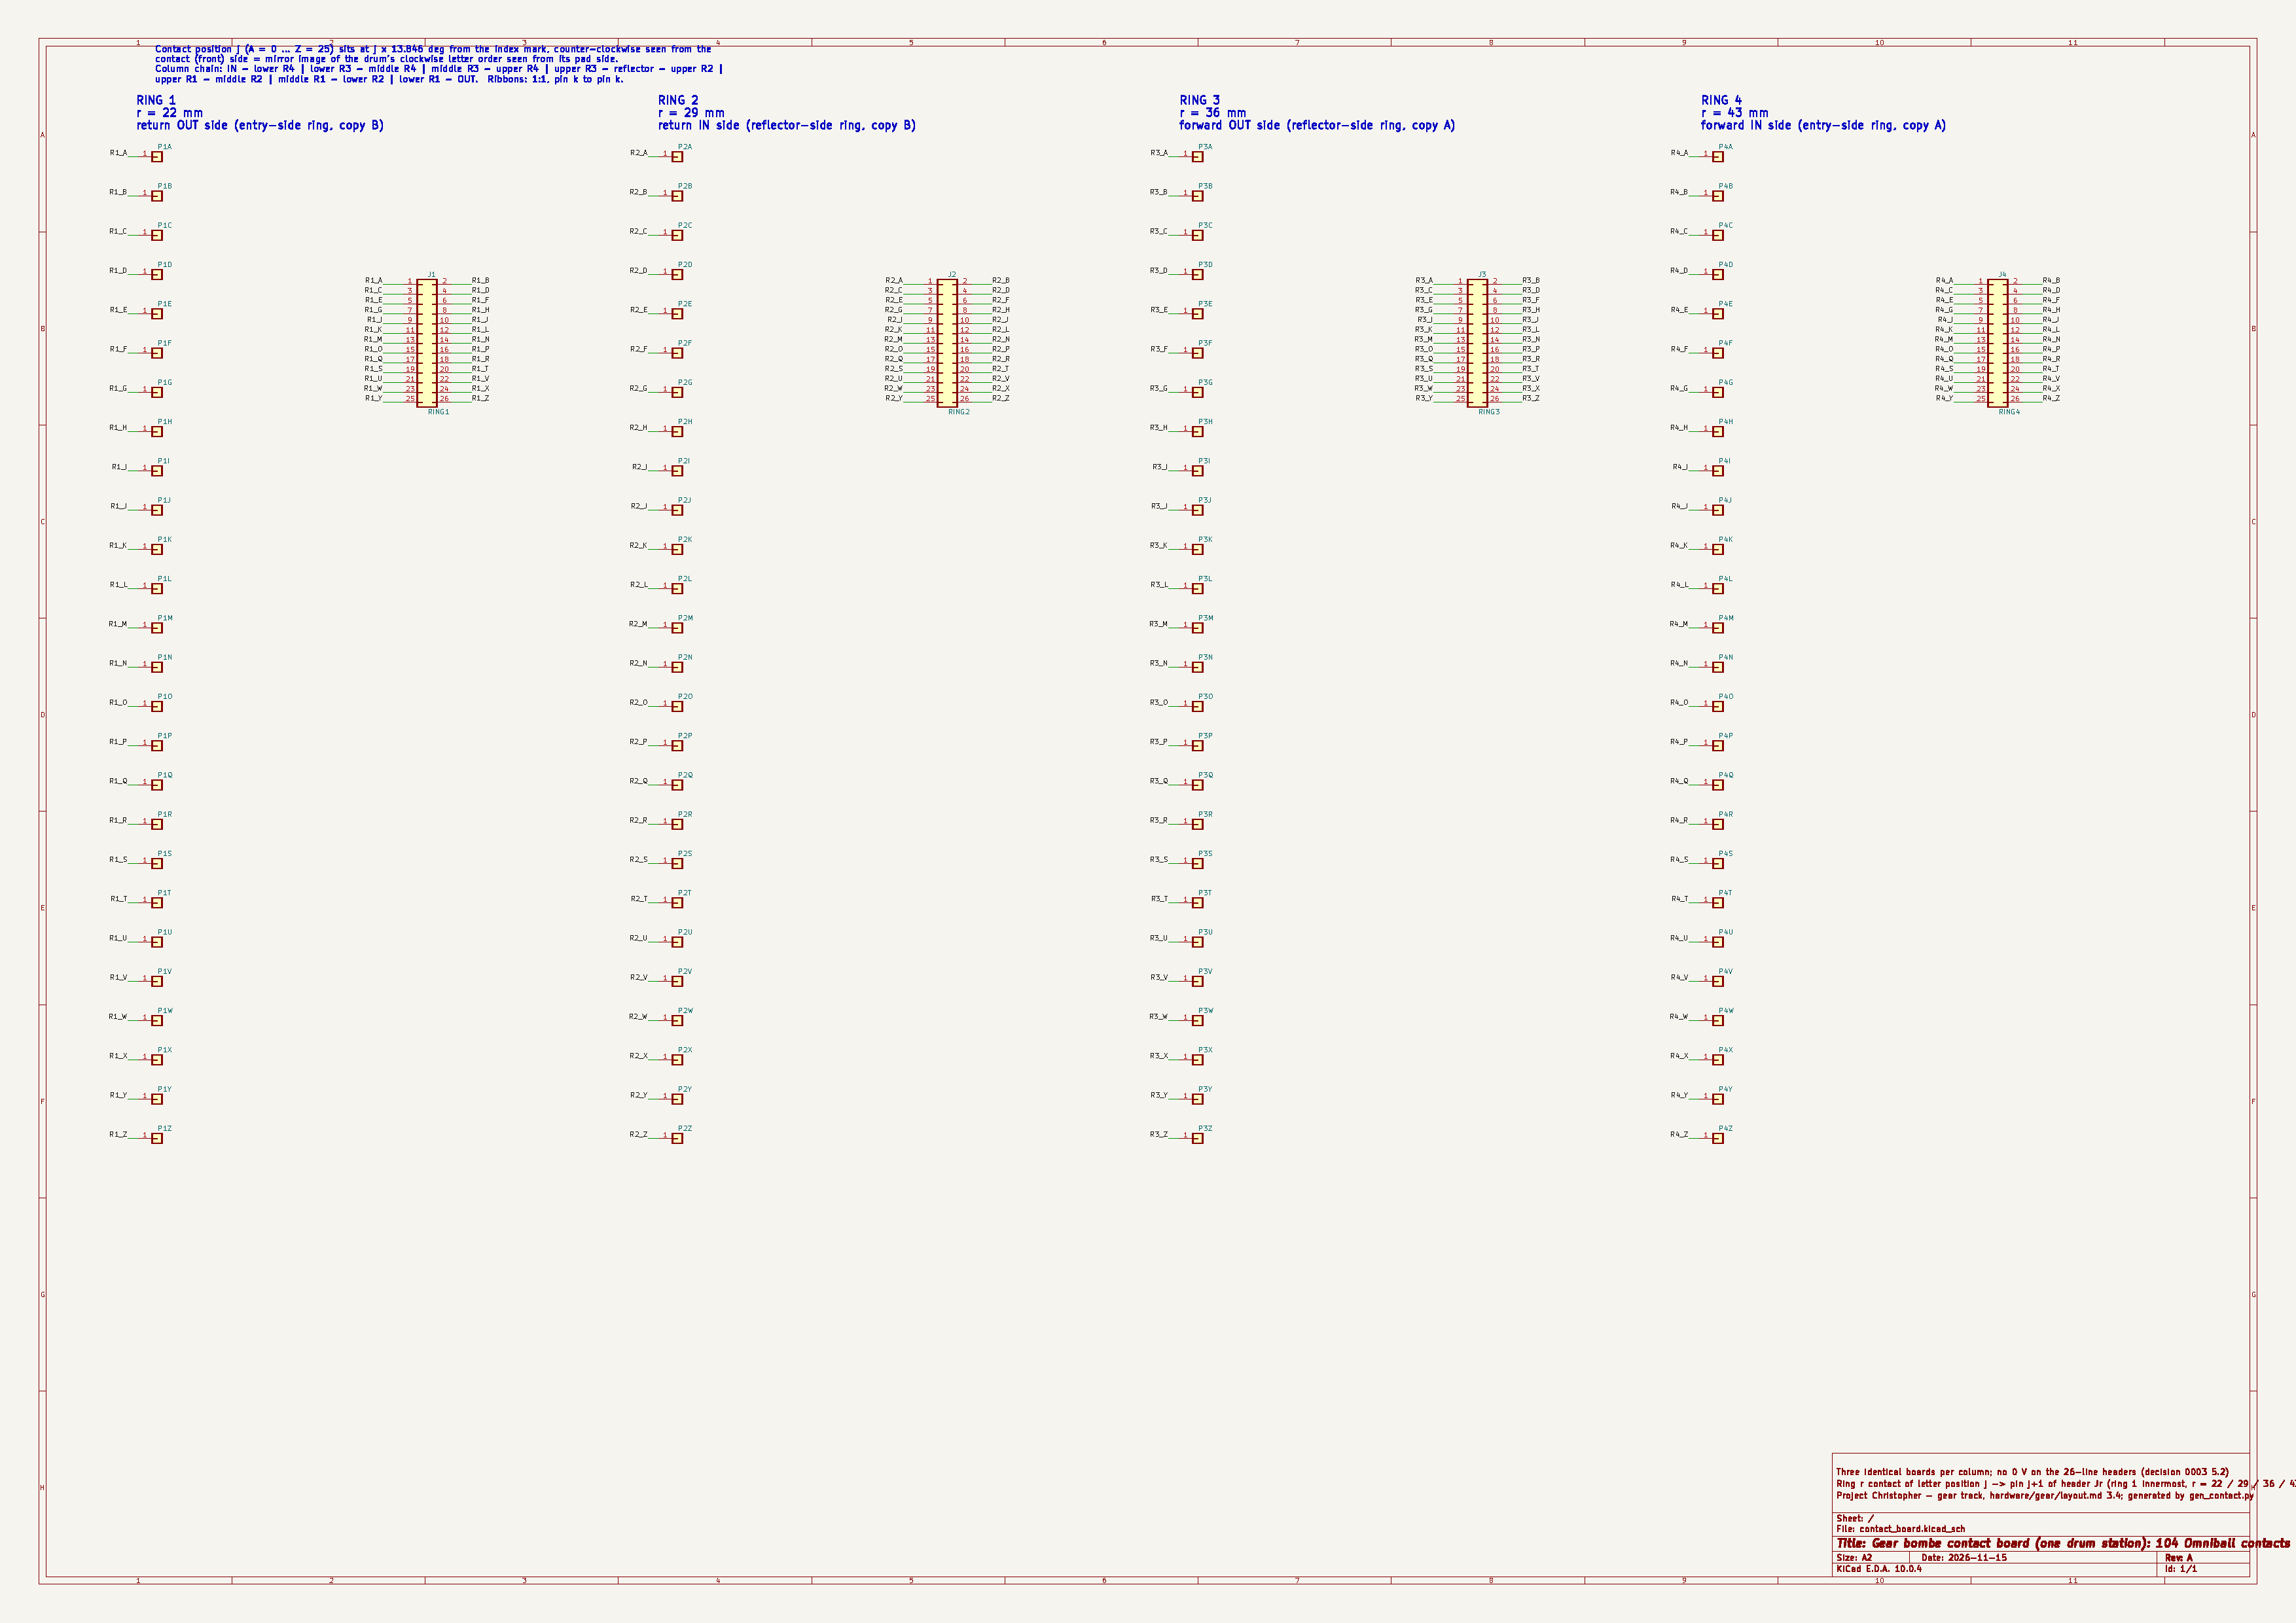
\includepdf[pages=-,pagecommand={\thispagestyle{plain}}]{figures/generated/sch_contact-board.pdf}}{}
\IfFileExists{figures/generated/sch_column-terminal.pdf}{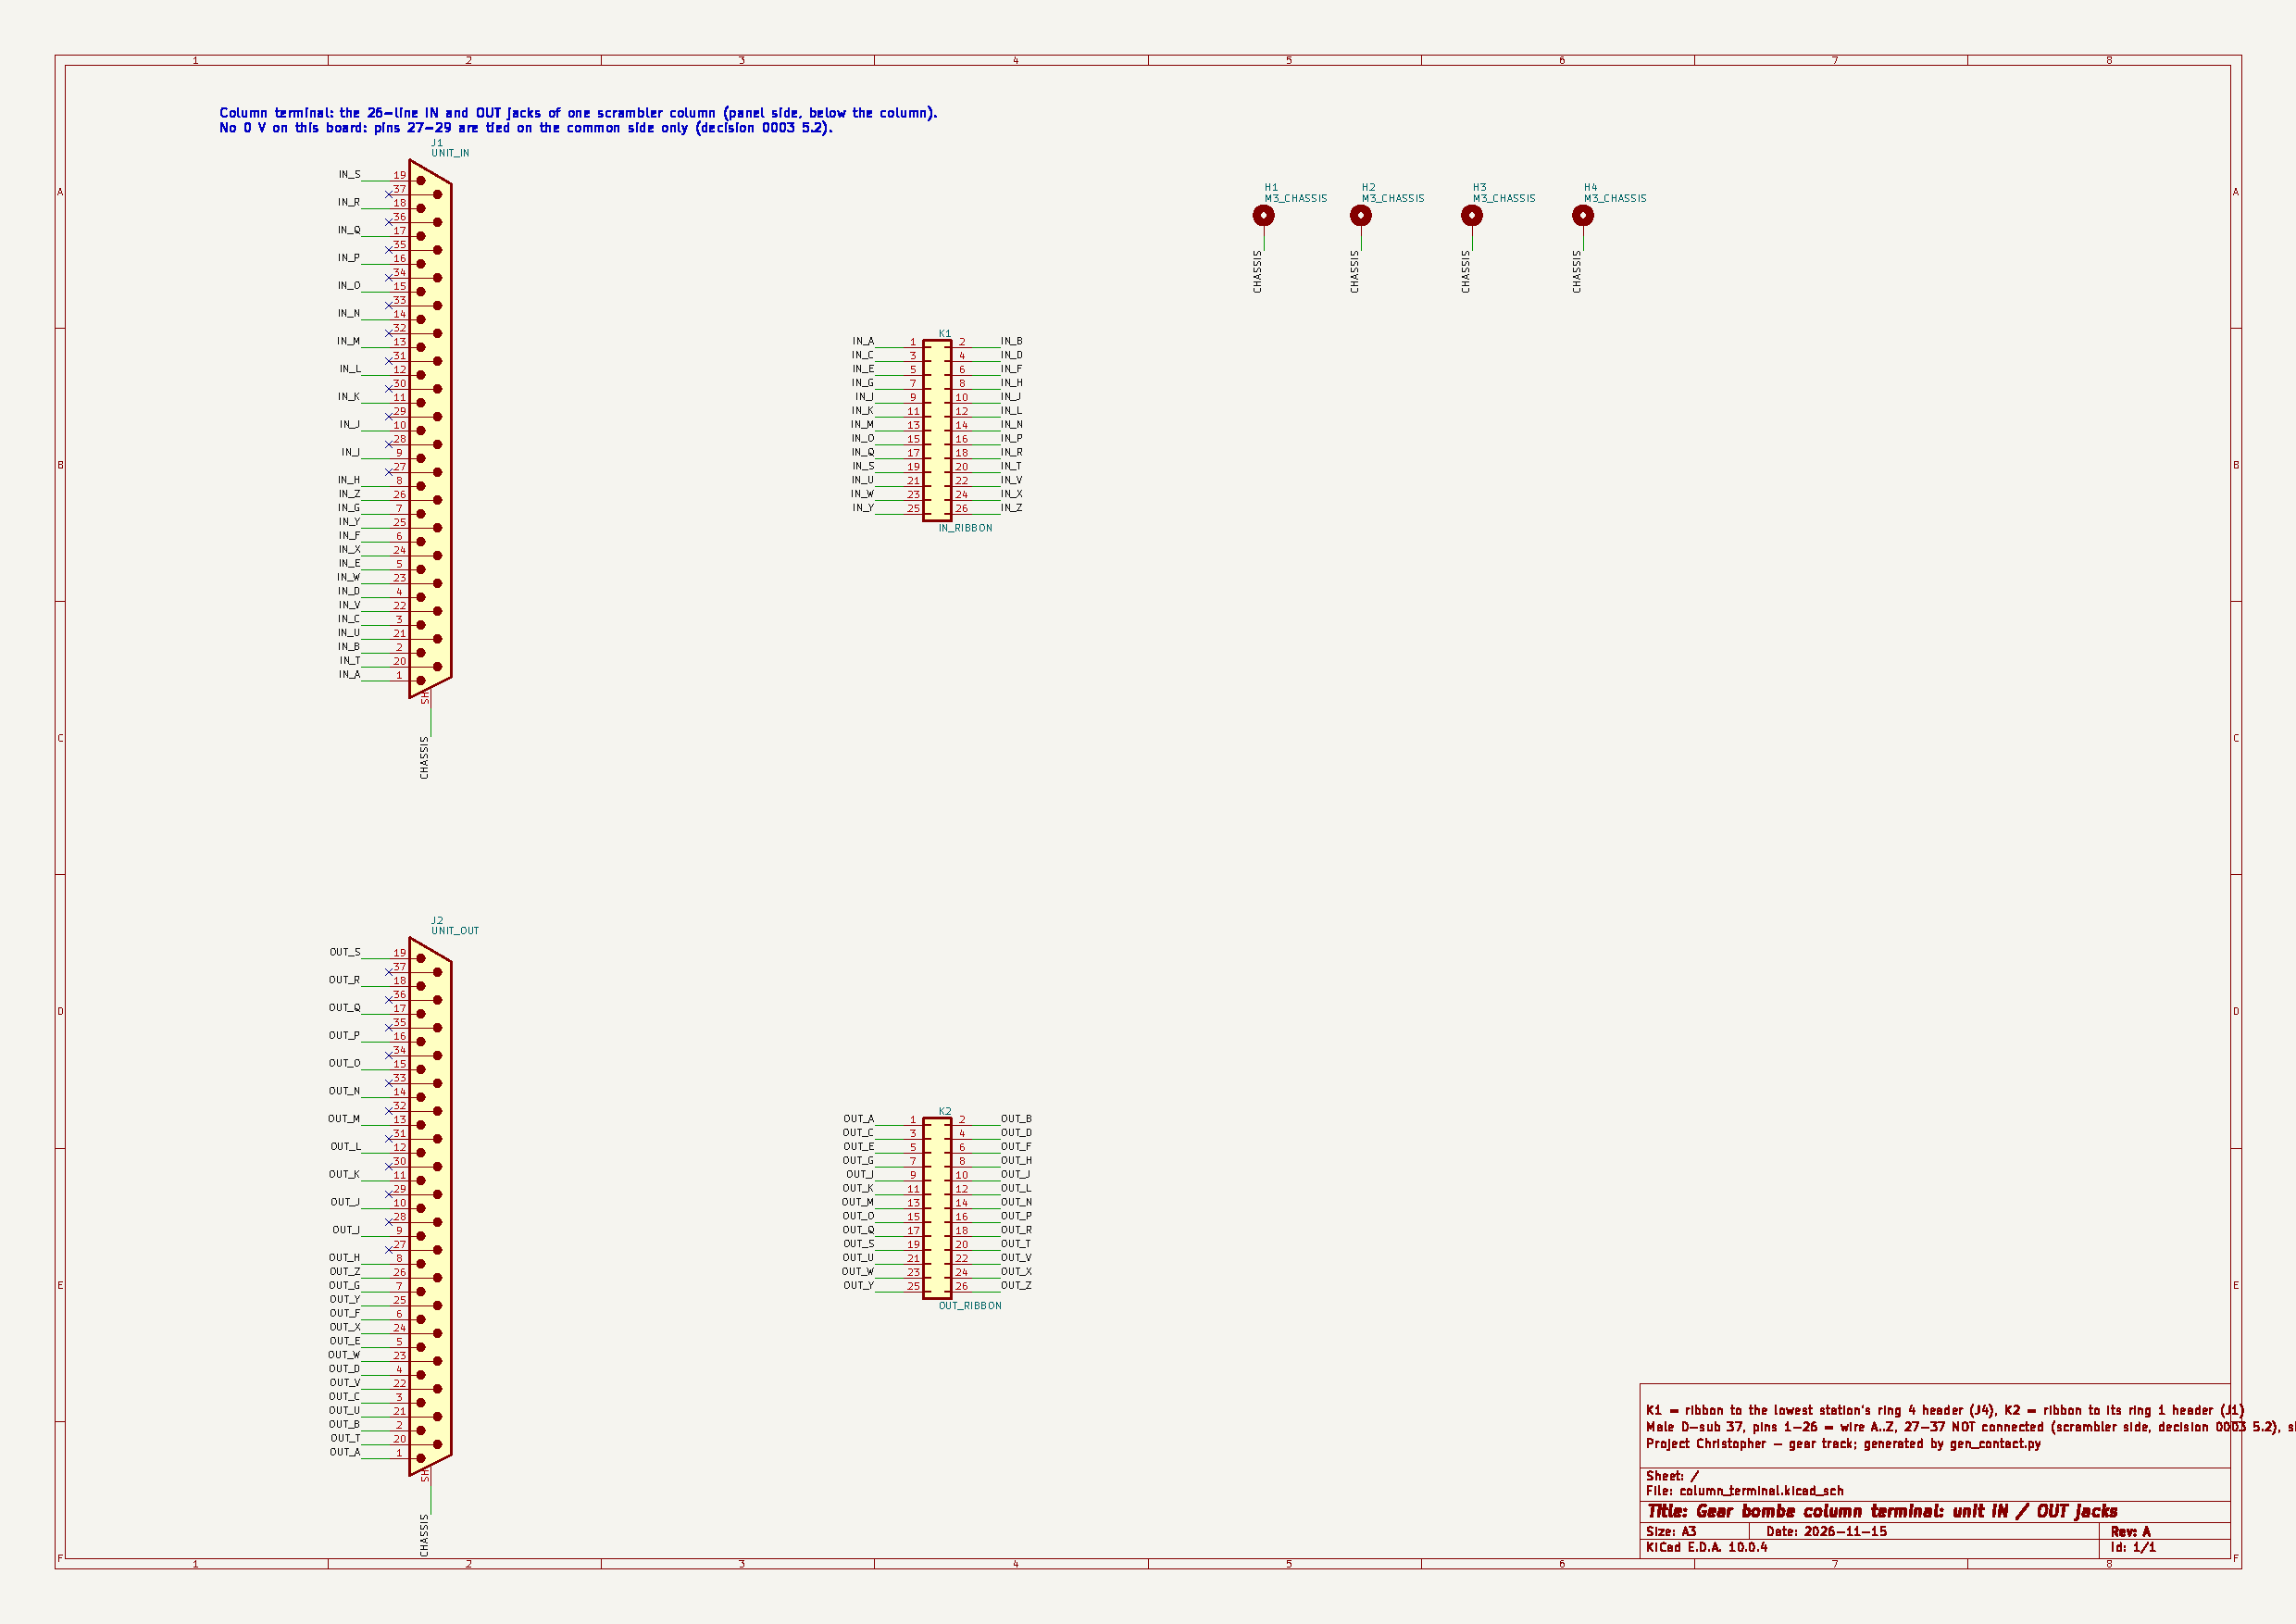
\includepdf[pages=-,pagecommand={\thispagestyle{plain}}]{figures/generated/sch_column-terminal.pdf}}{}
\IfFileExists{figures/generated/sch_reflector-card-b.pdf}{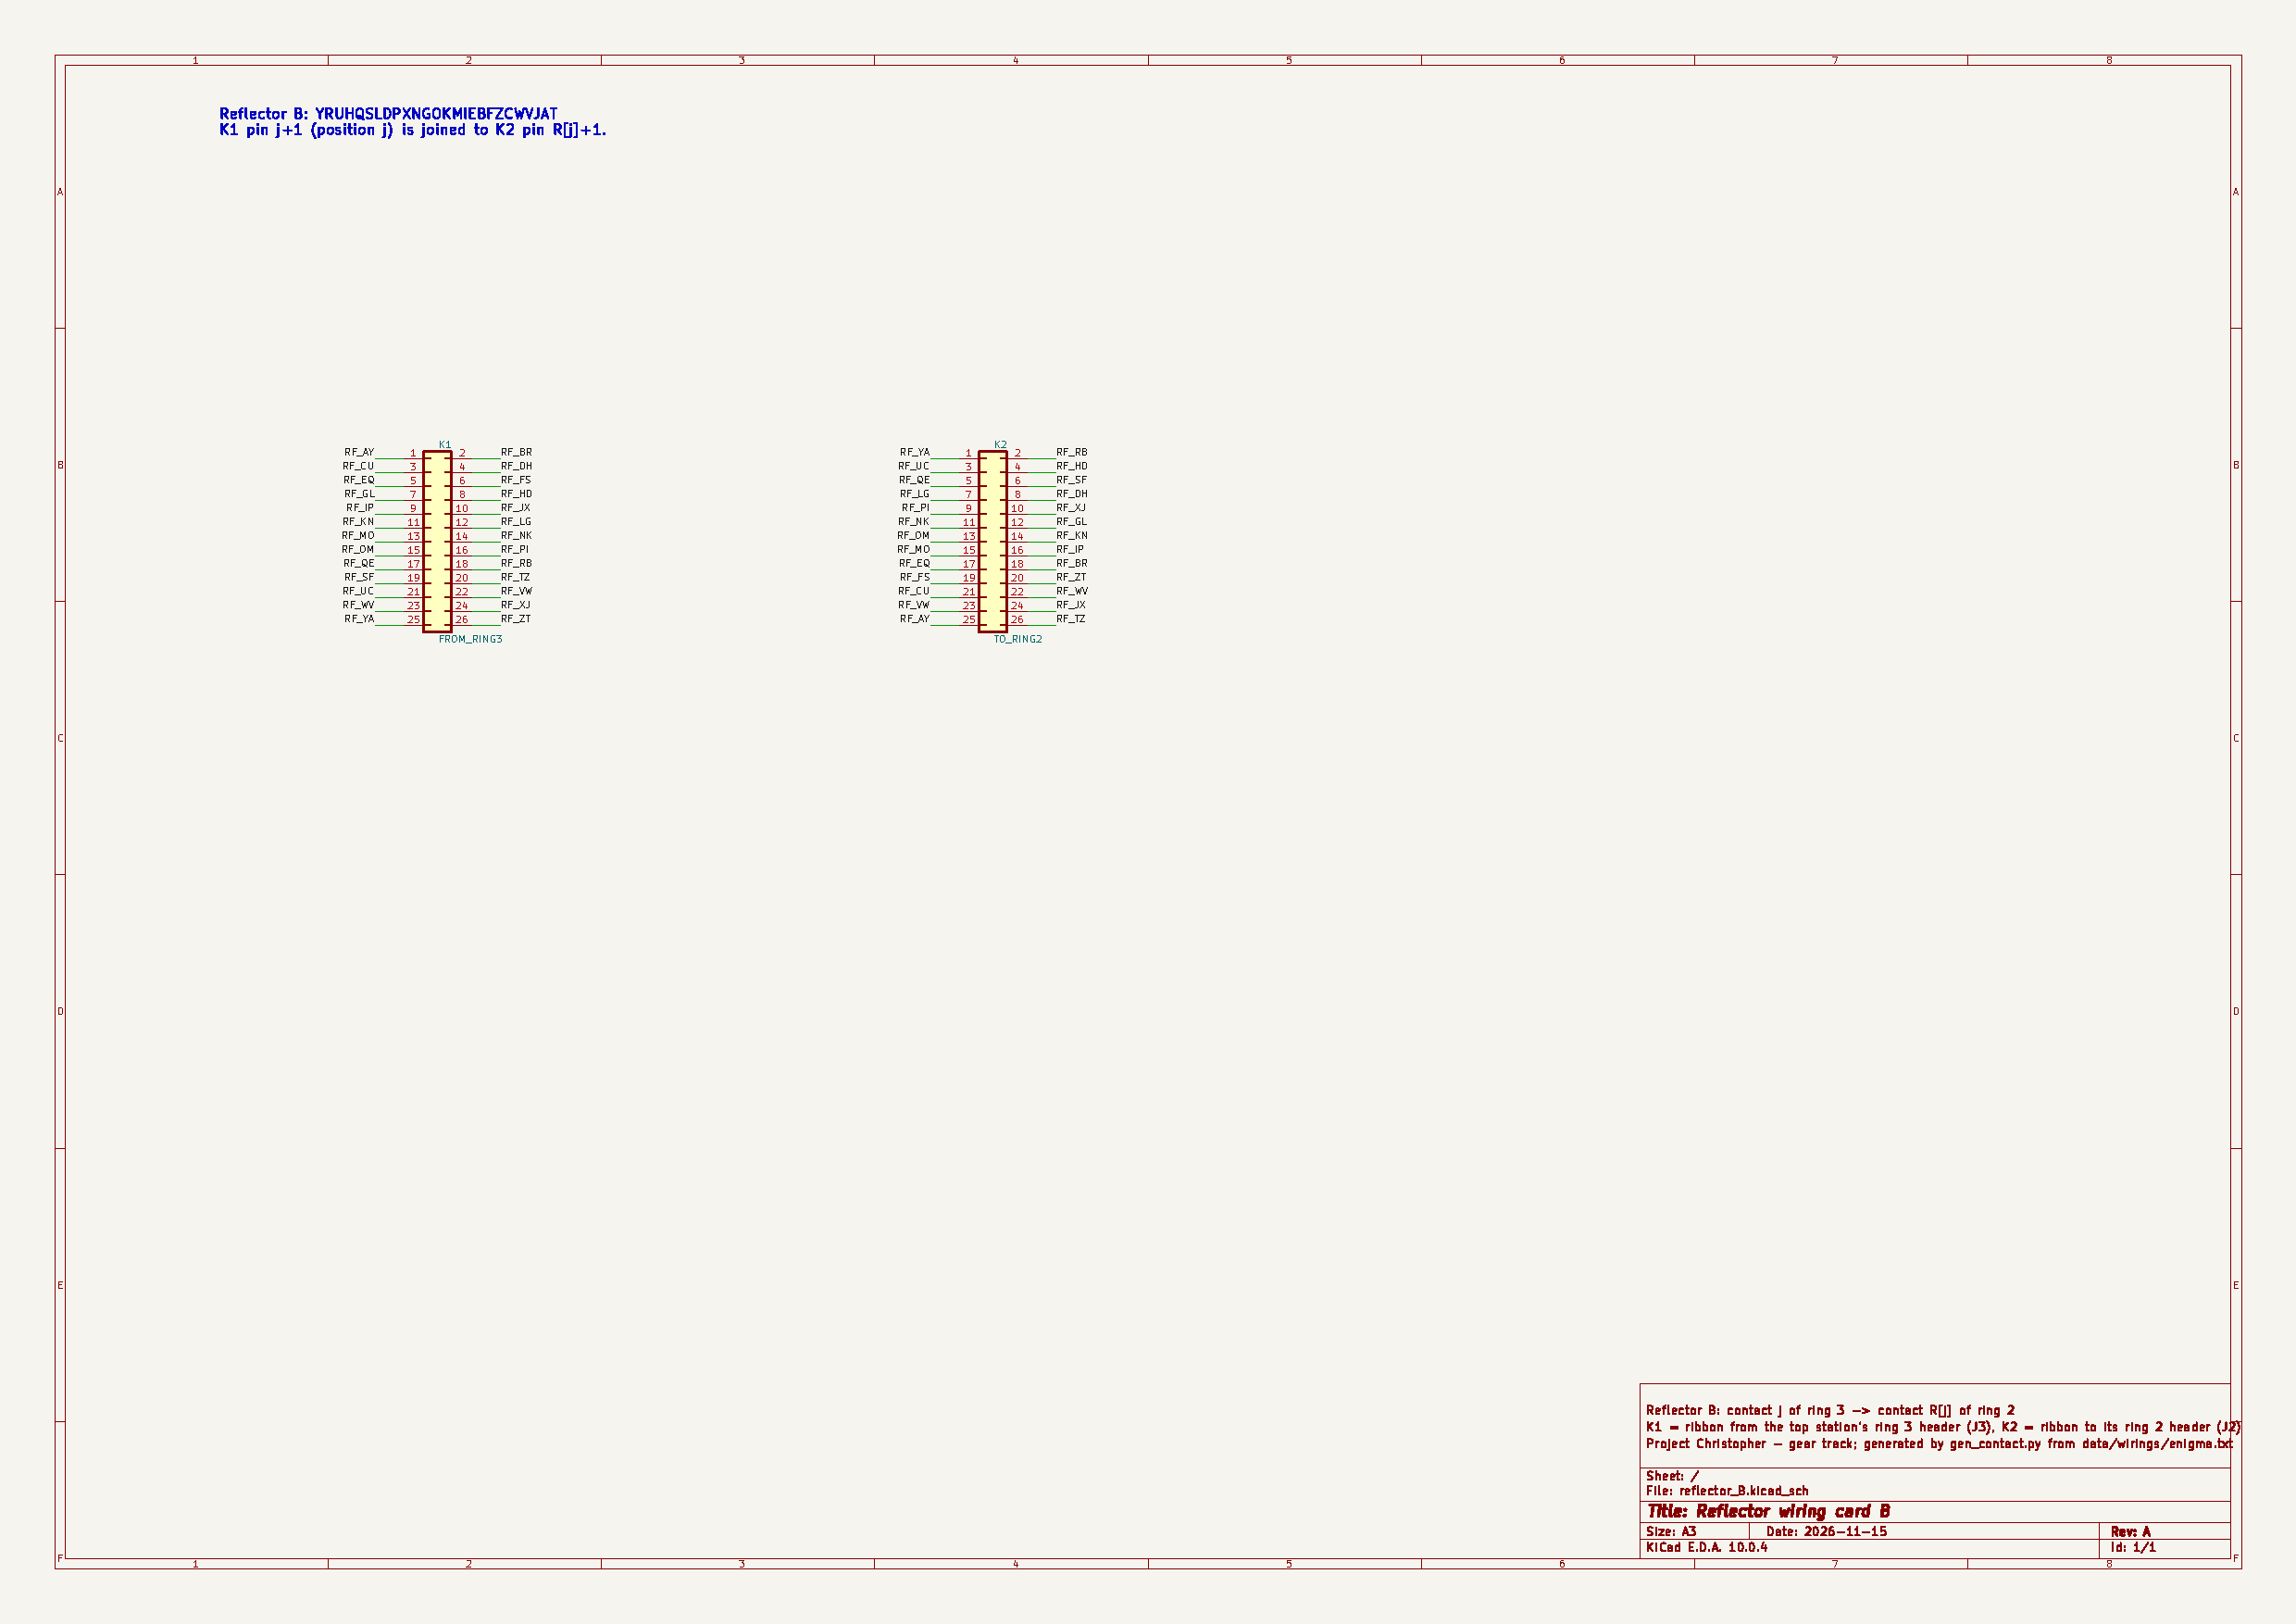
\includepdf[pages=-,pagecommand={\thispagestyle{plain}}]{figures/generated/sch_reflector-card-b.pdf}}{}

\section{대각선 보드(다섯 장)}\label{sch:diagonal}
글자 6/6/6/4/4개씩 나눈 다섯 장(D1--D5). 글자마다 수 D-sub 37 잭 두 개, 보드 사이는 64핀 IDC 세 가닥이다.
\code{hardware/common/diagonal-board/verify\_diagonal.py}가 다섯 넷리스트를 접속 리본으로 합쳐, 대각선 연결
325개(선 $w$의 글자 $c$ ↔ 선 $c$의 글자 $w$)가 정확히 그것만 이어지고 27--29번 0\,V가 한 넷임을 확인했다.
\IfFileExists{figures/generated/sch_diagonal-d1.pdf}{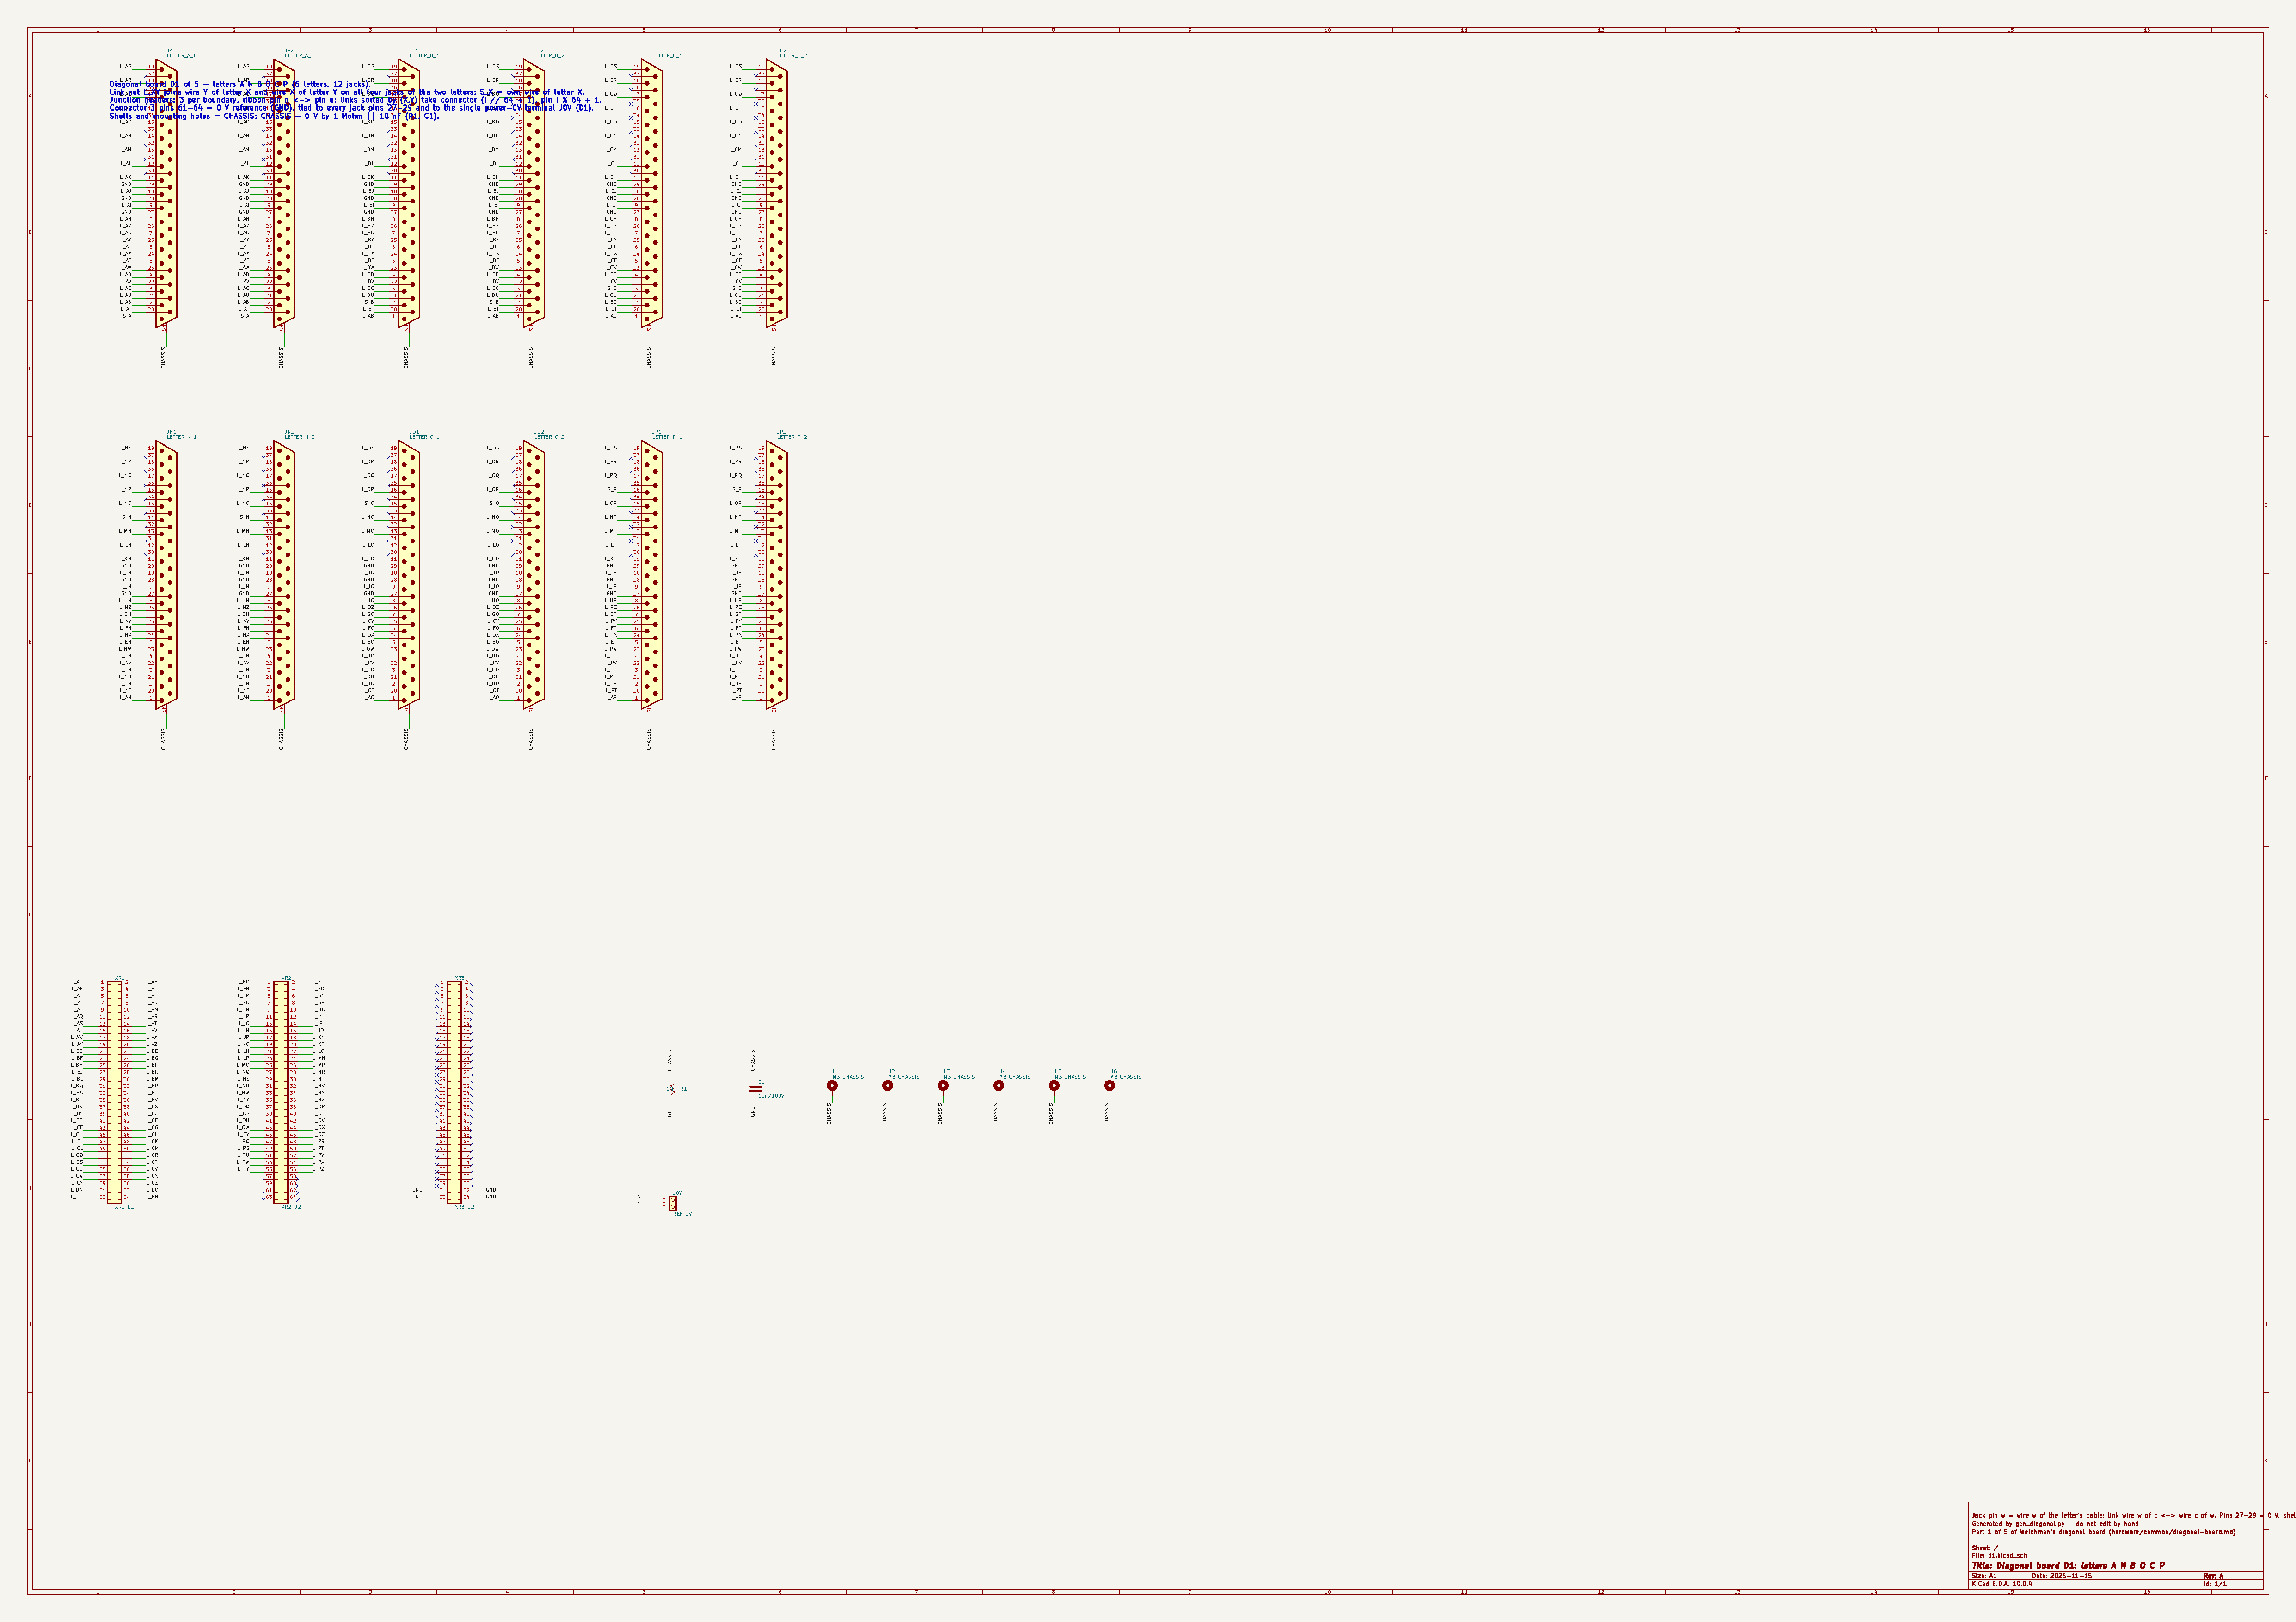
\includepdf[pages=-,pagecommand={\thispagestyle{plain}}]{figures/generated/sch_diagonal-d1.pdf}}{}
\IfFileExists{figures/generated/sch_diagonal-d2.pdf}{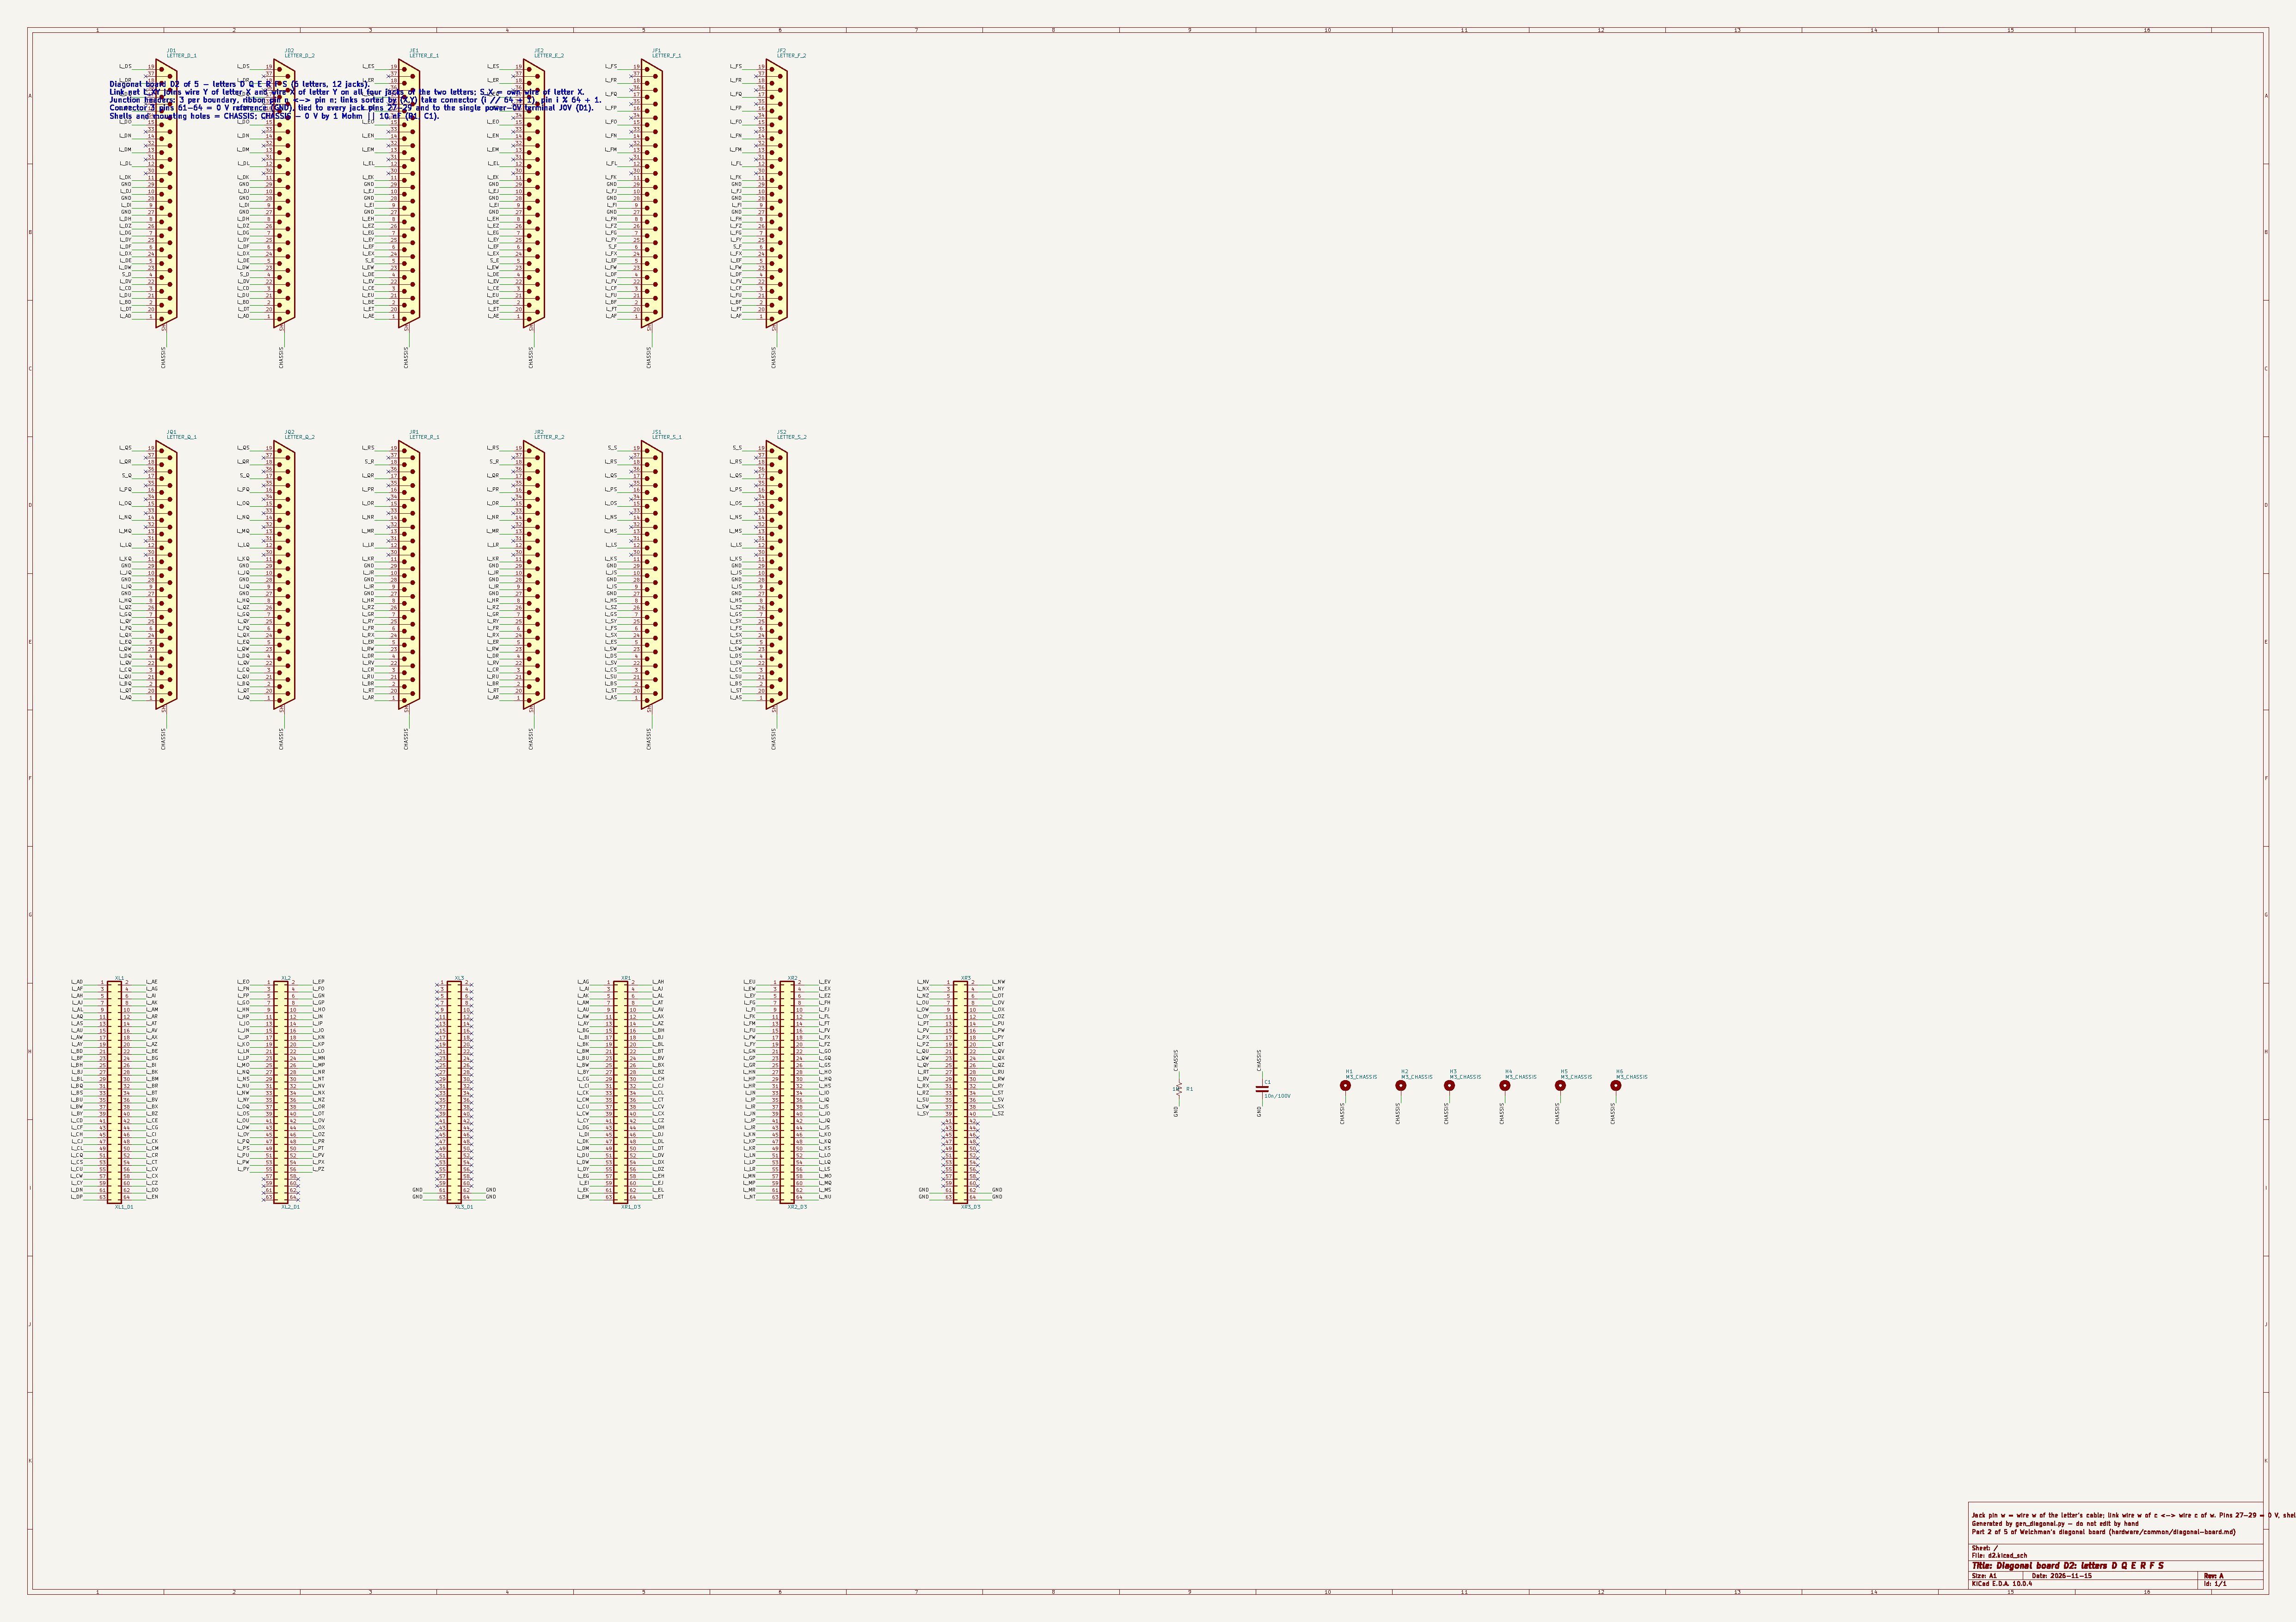
\includepdf[pages=-,pagecommand={\thispagestyle{plain}}]{figures/generated/sch_diagonal-d2.pdf}}{}
\IfFileExists{figures/generated/sch_diagonal-d3.pdf}{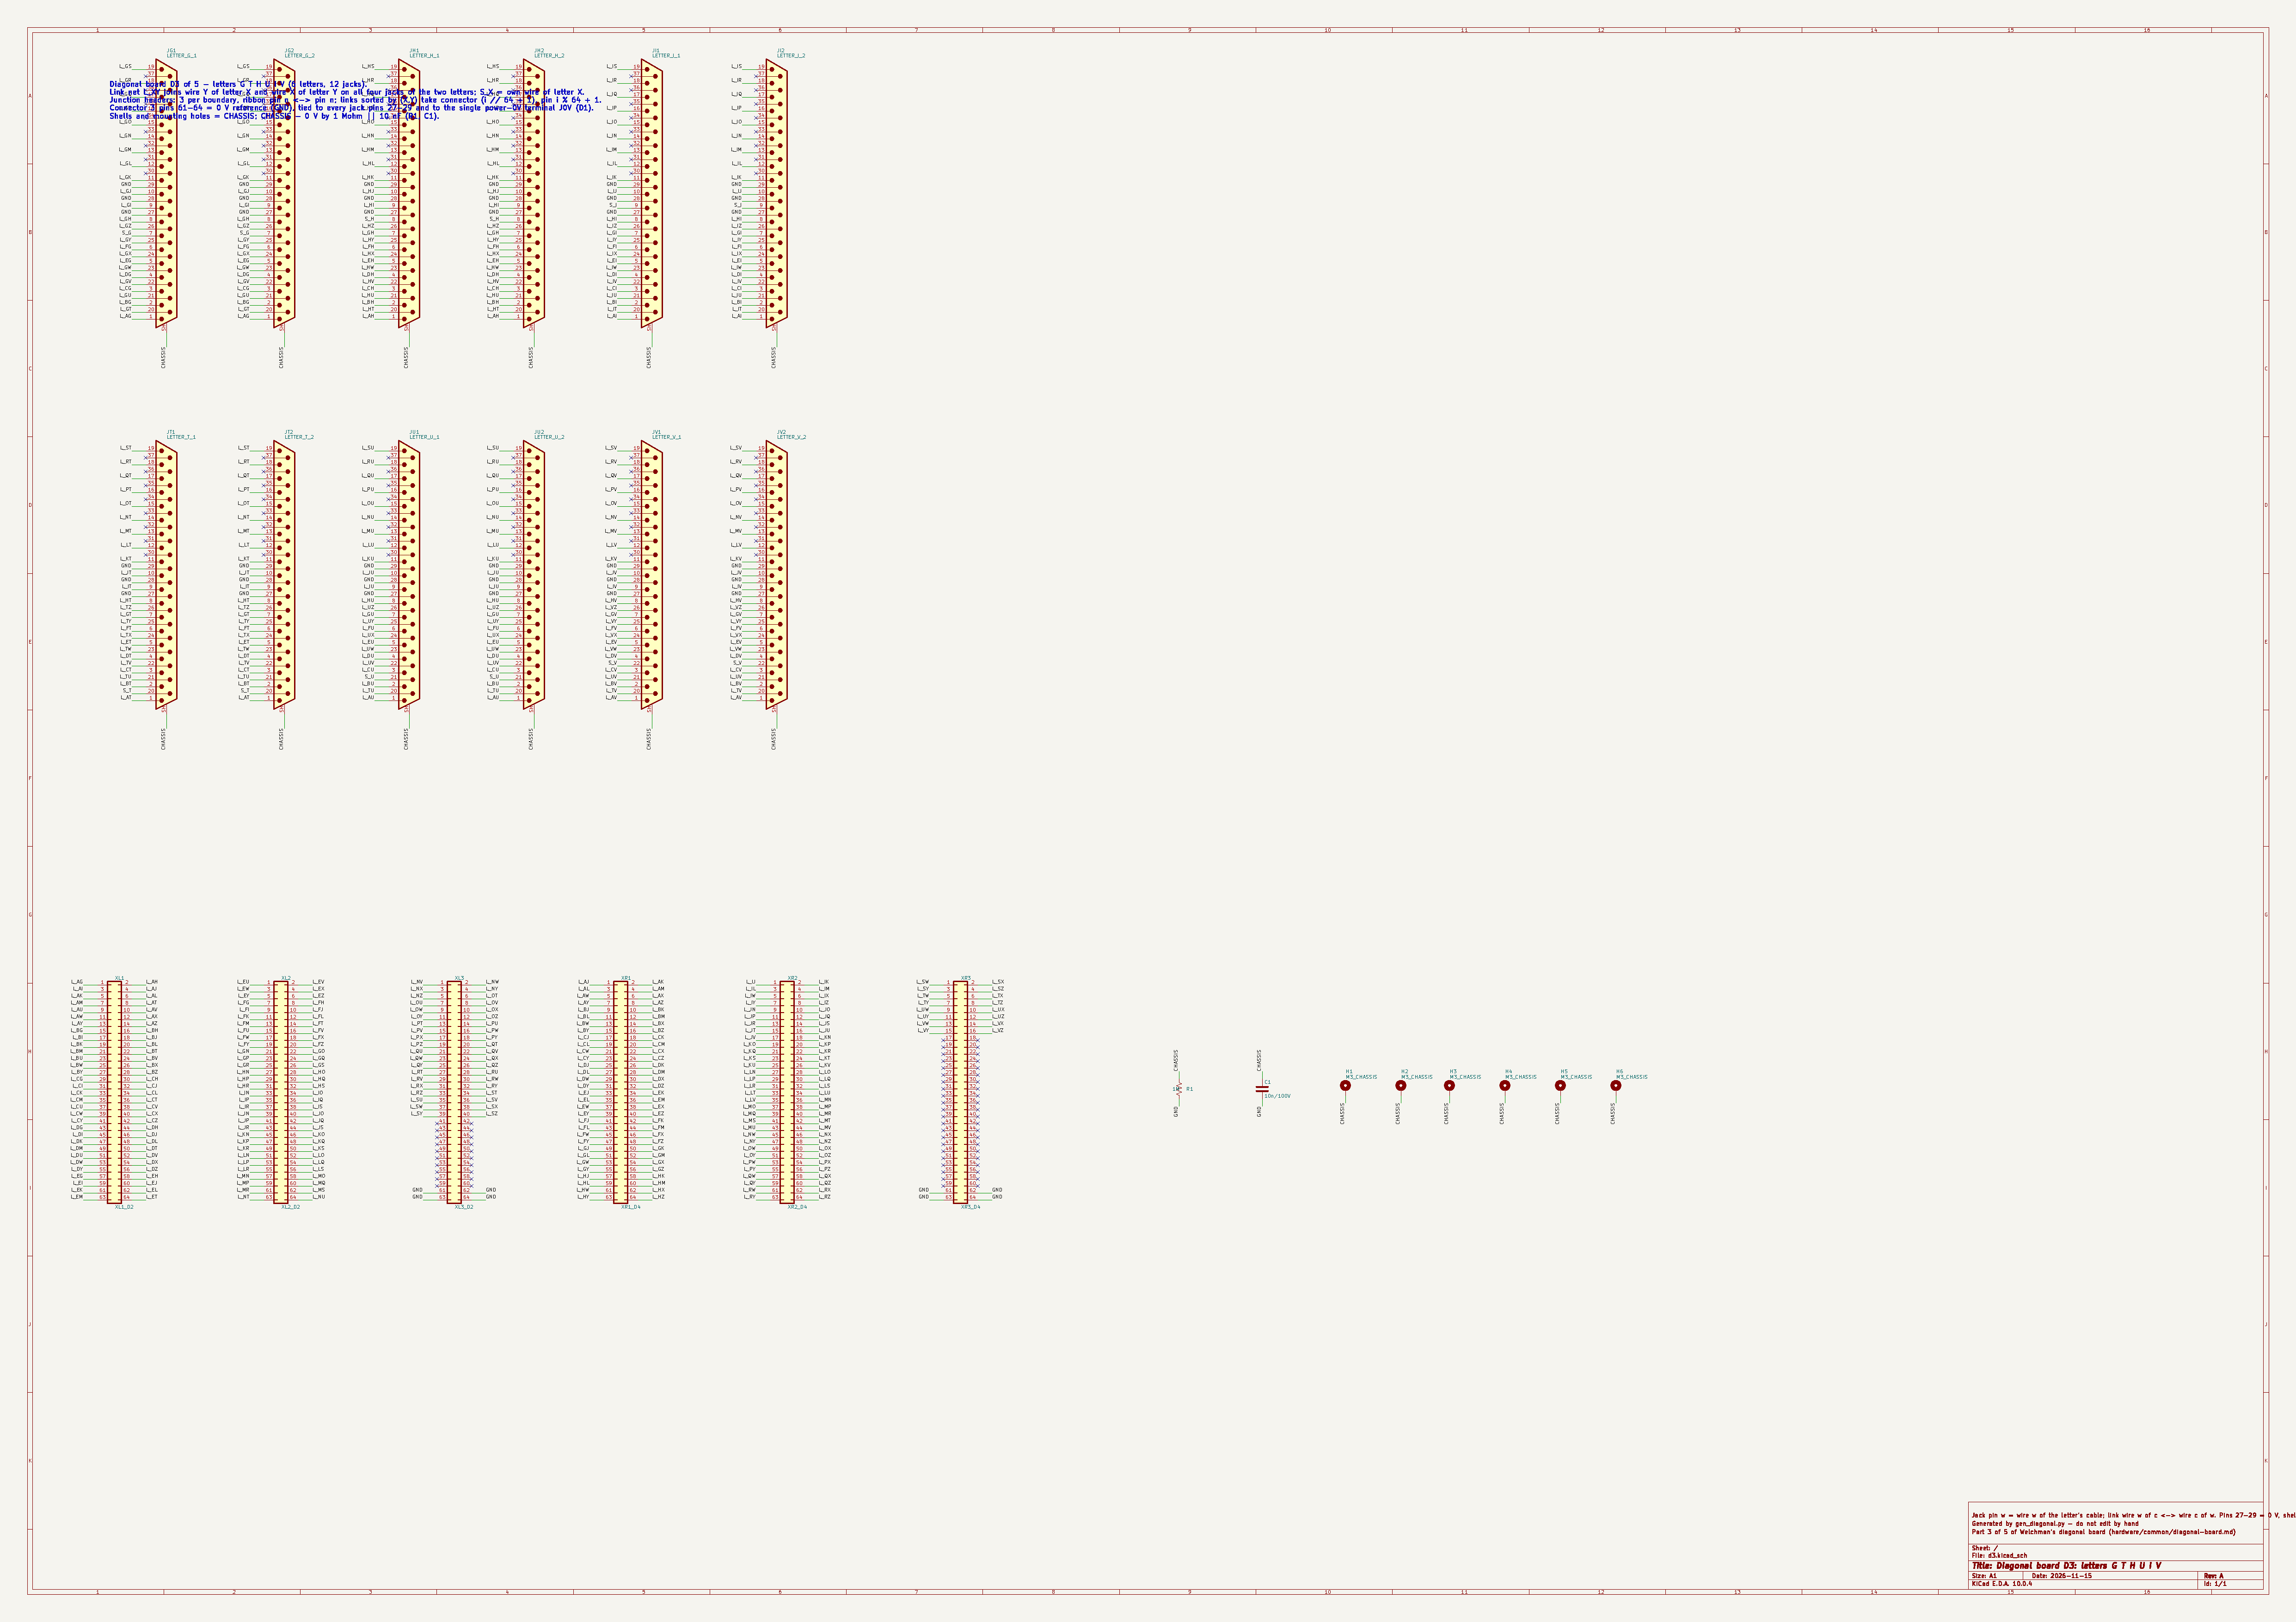
\includepdf[pages=-,pagecommand={\thispagestyle{plain}}]{figures/generated/sch_diagonal-d3.pdf}}{}
\IfFileExists{figures/generated/sch_diagonal-d4.pdf}{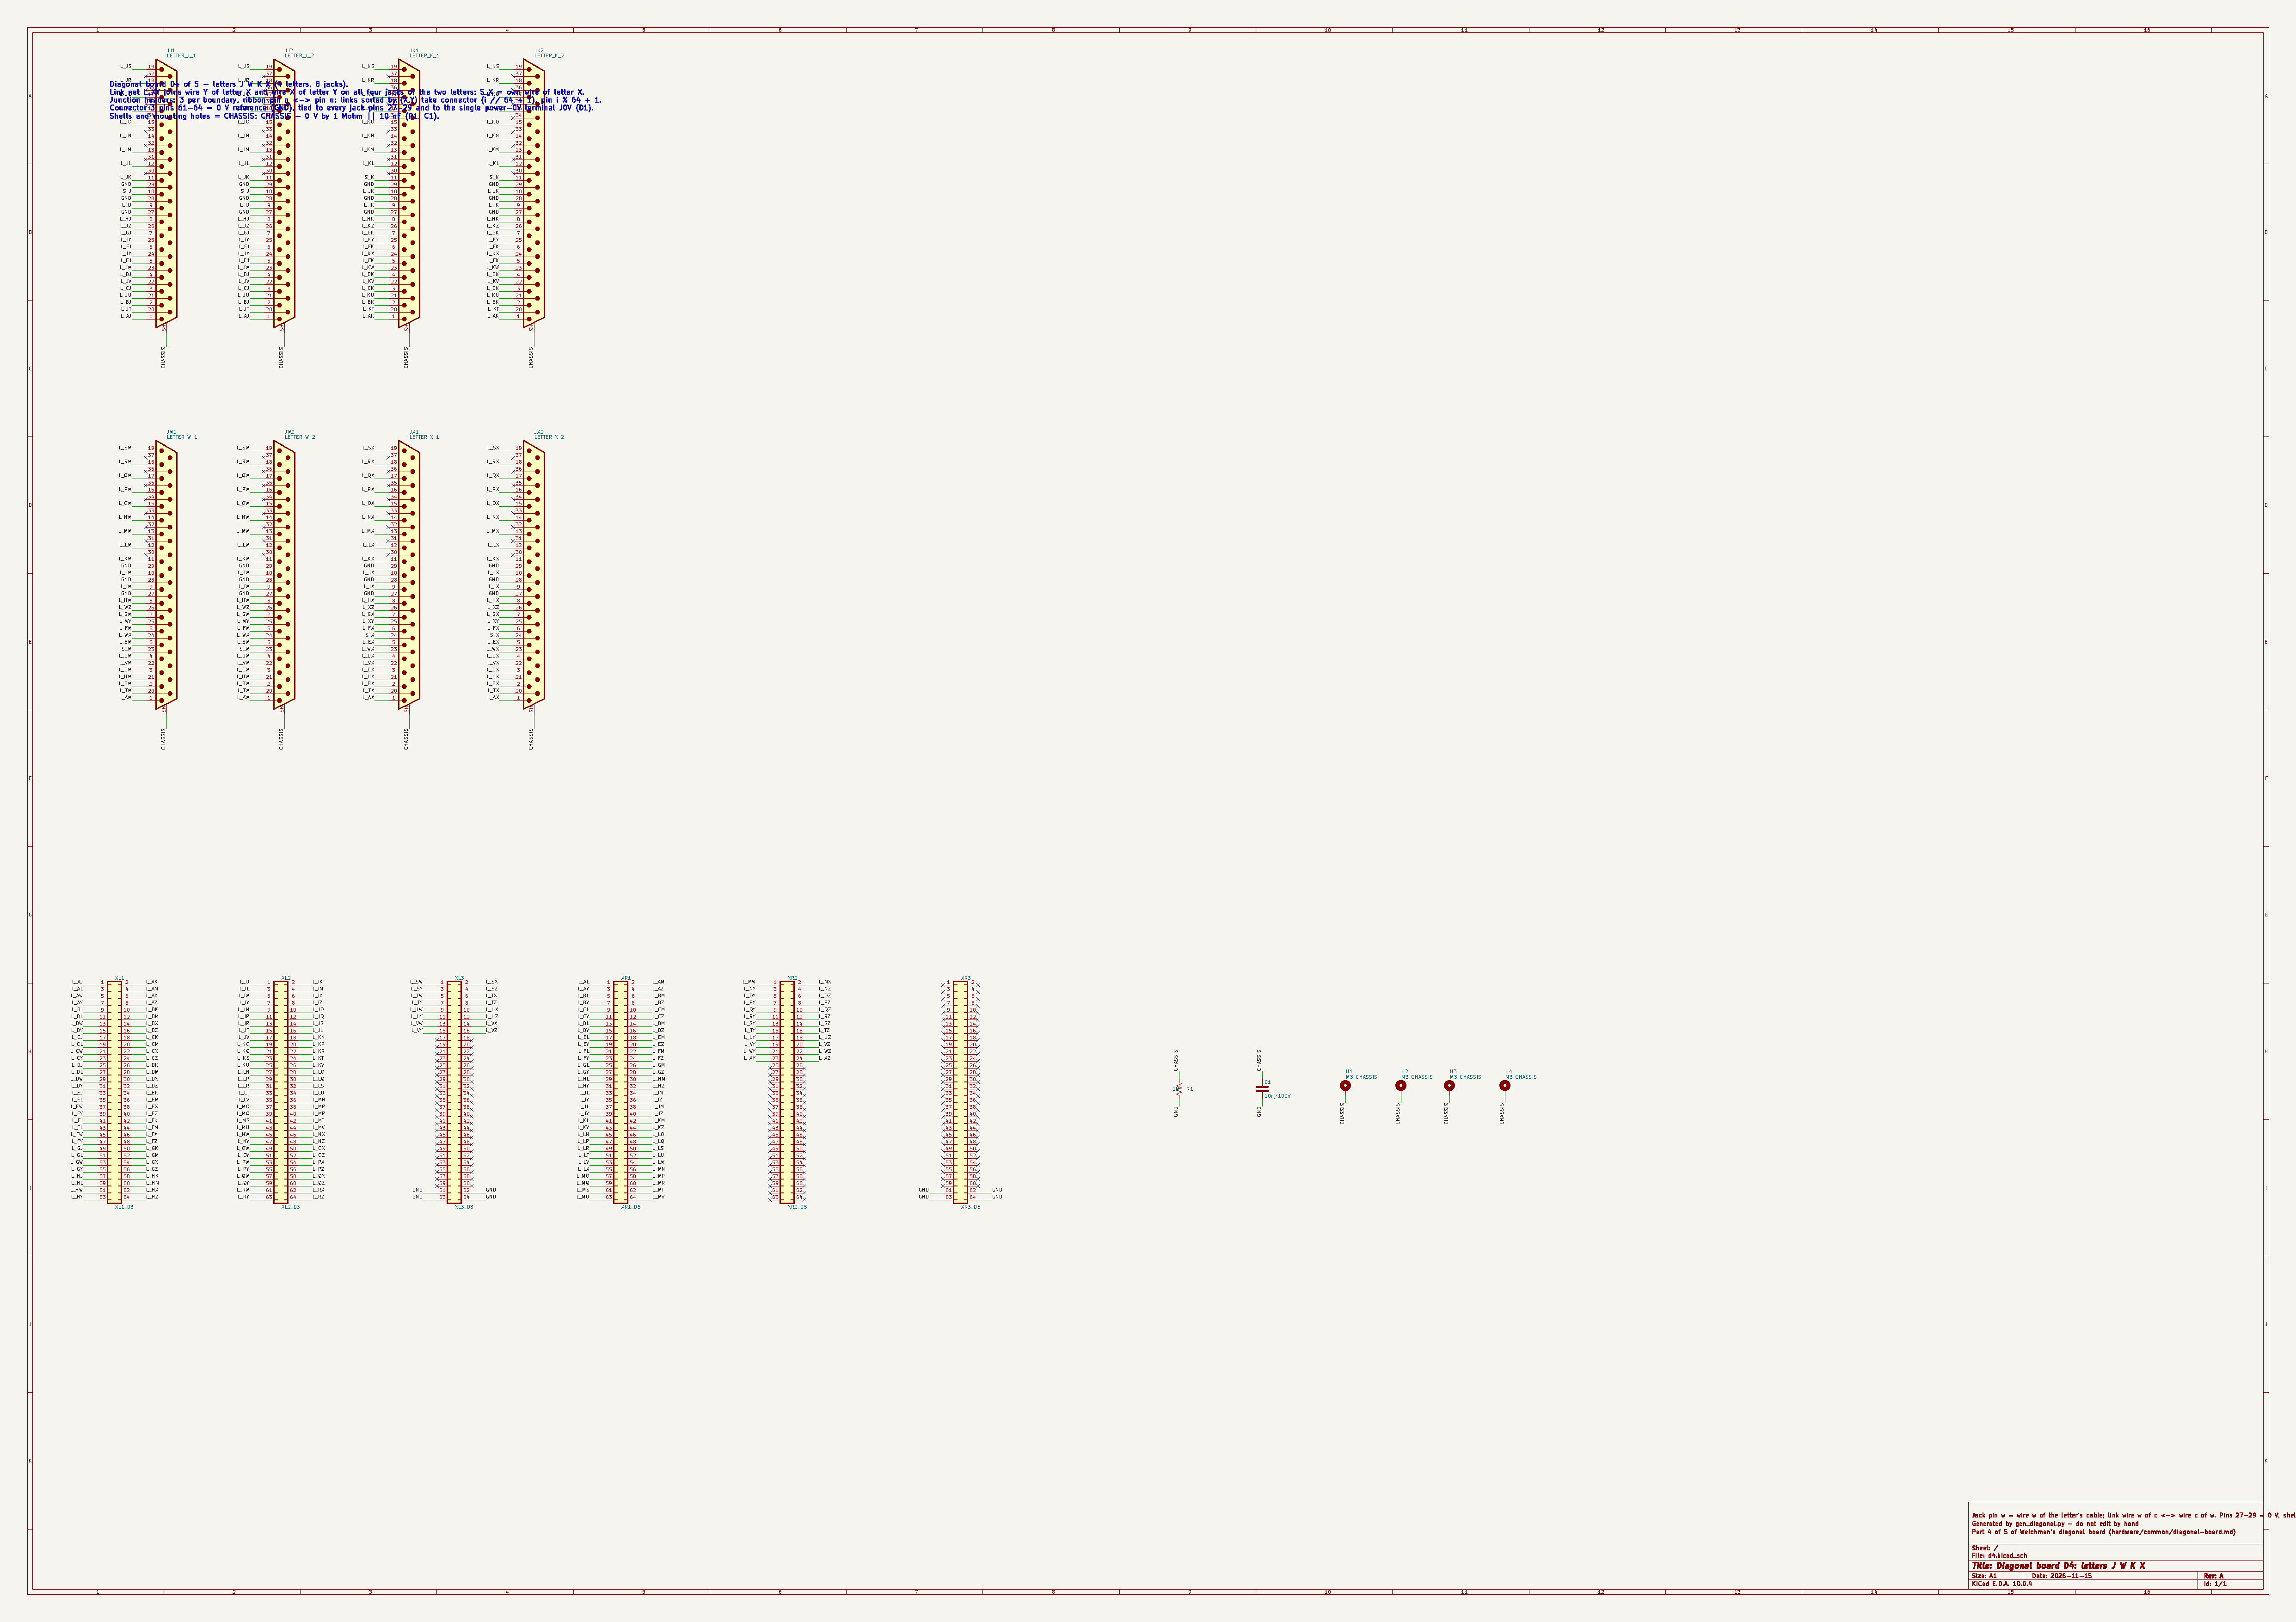
\includepdf[pages=-,pagecommand={\thispagestyle{plain}}]{figures/generated/sch_diagonal-d4.pdf}}{}
\IfFileExists{figures/generated/sch_diagonal-d5.pdf}{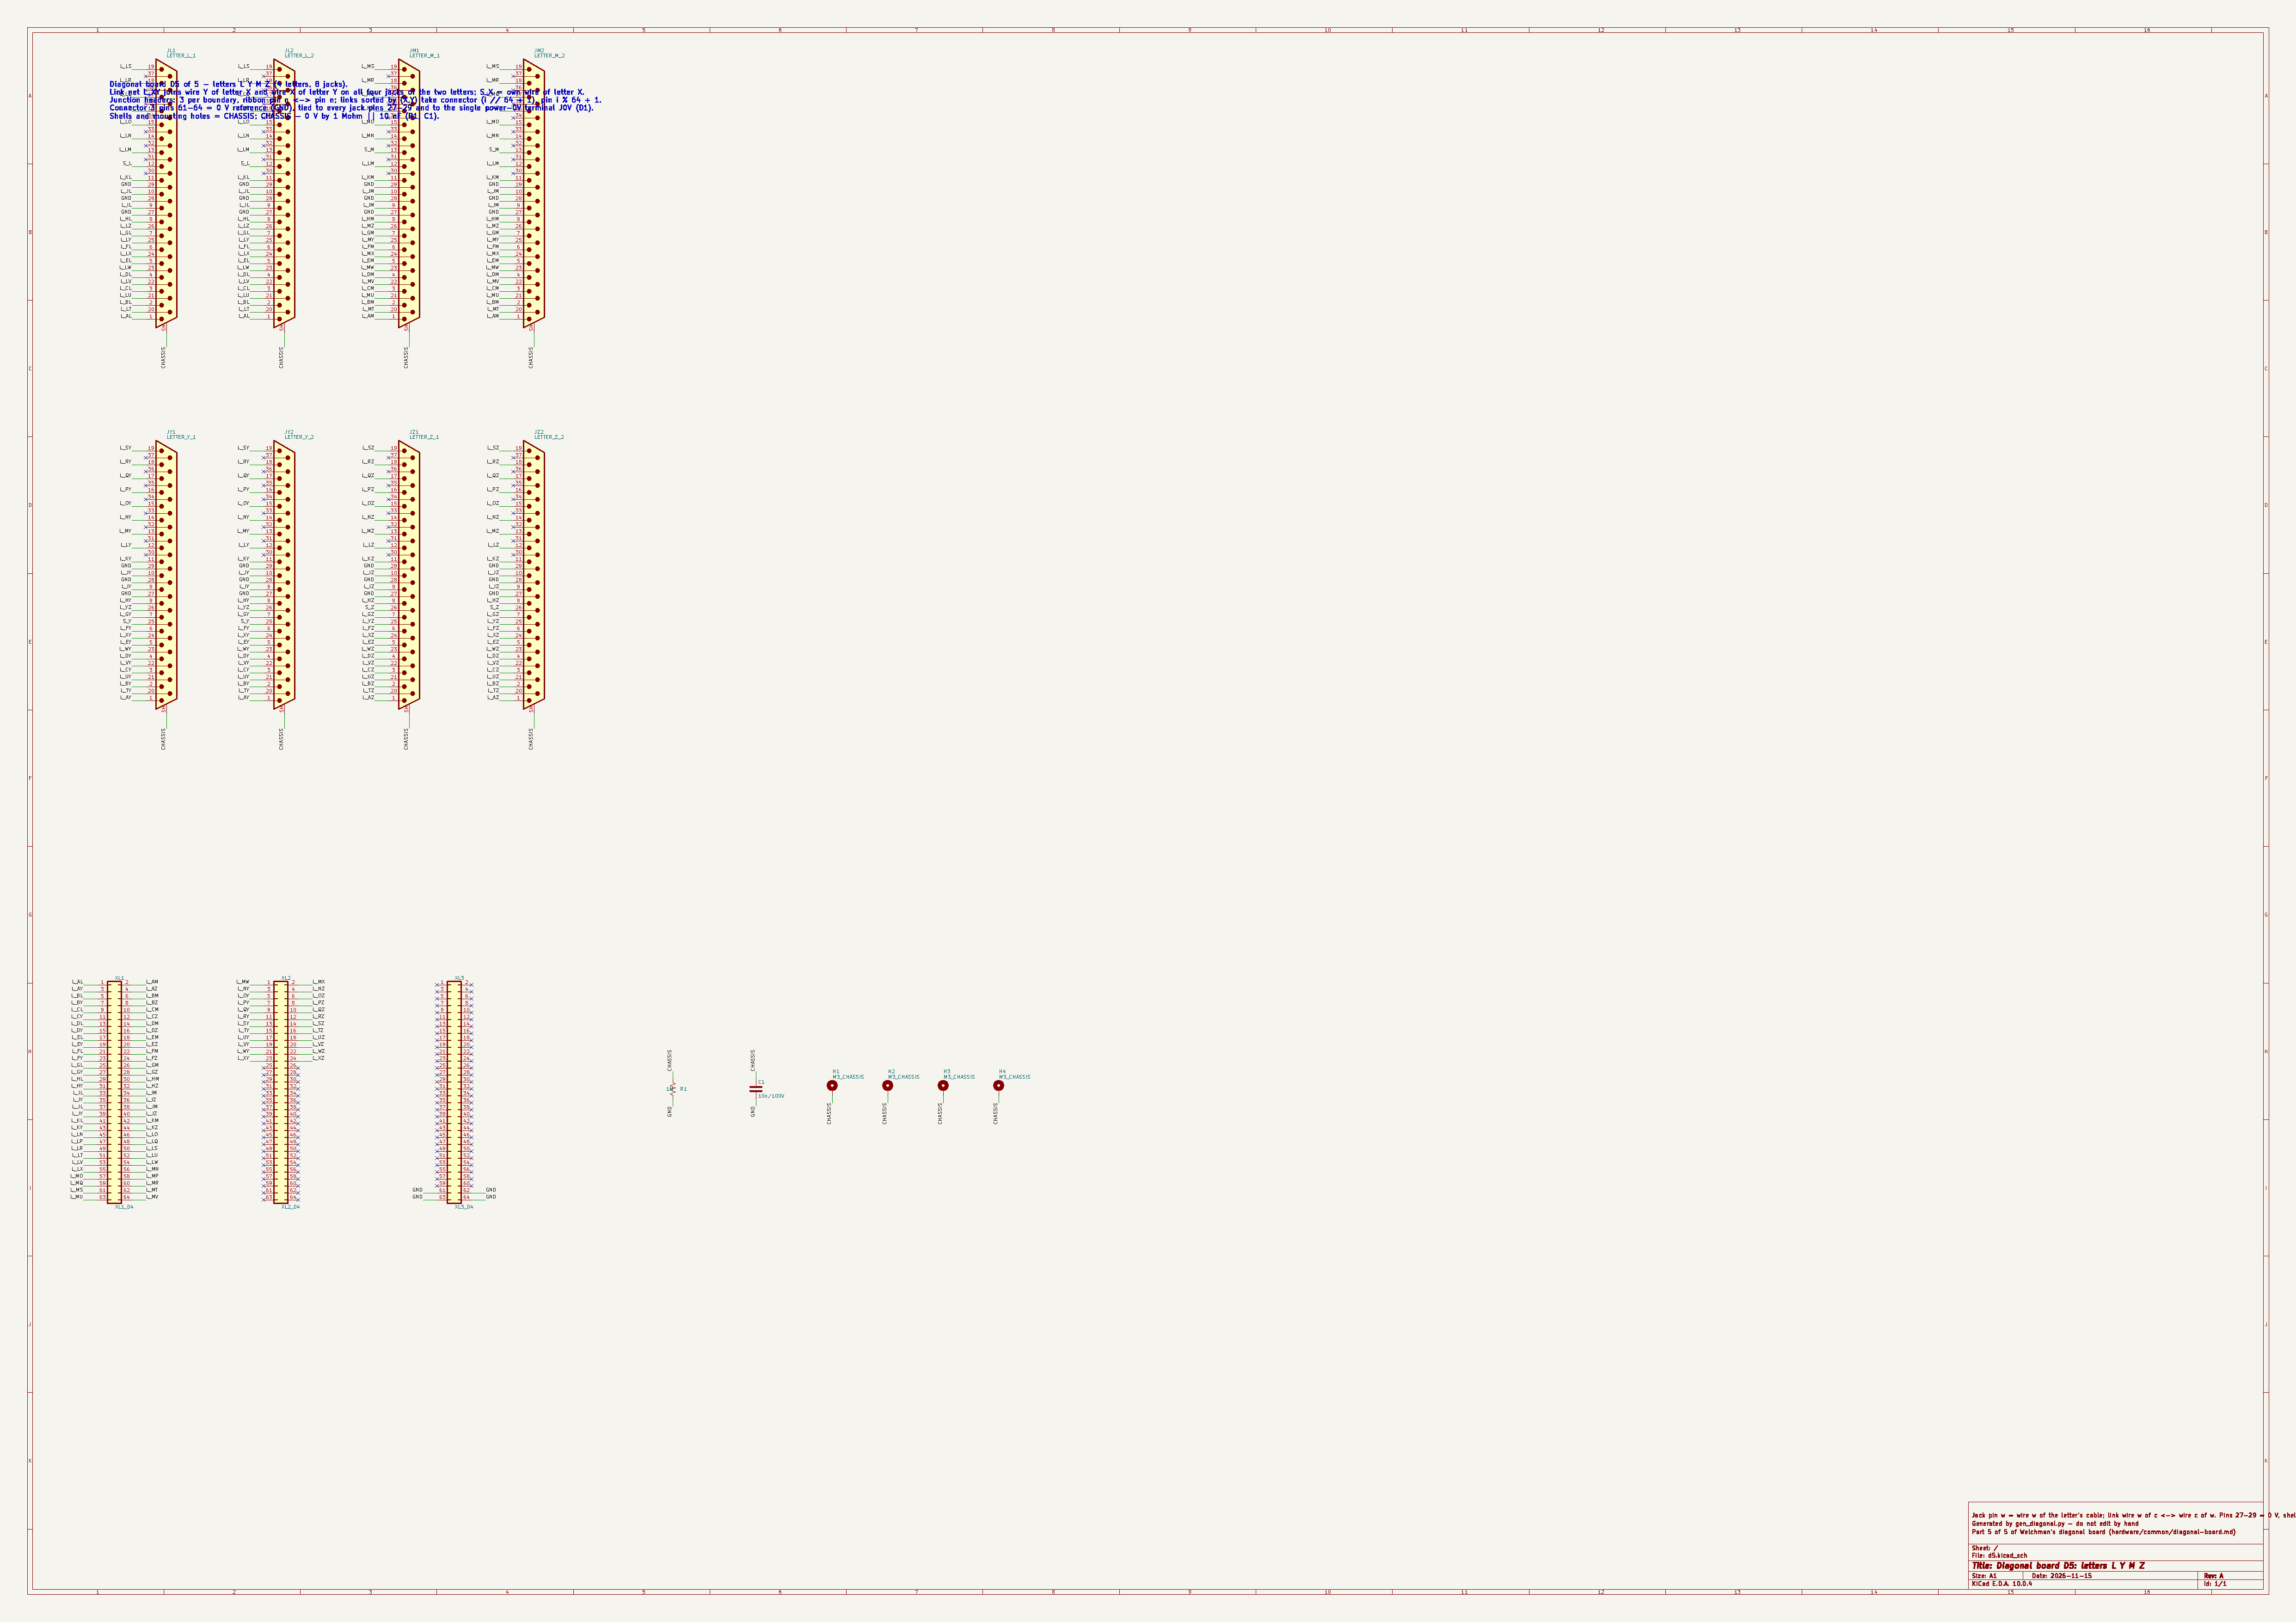
\includepdf[pages=-,pagecommand={\thispagestyle{plain}}]{figures/generated/sch_diagonal-d5.pdf}}{}

\section{메뉴 패치 패널}\label{sch:patch-panel}
공통 잭 4묶음 × 4개, 테스트 레지스터 잭, 탐색 잭과 시험 전압 플러그를 꽂는 26구멍, 0\,V(27--29번)를 묶는 곳이다.
글자 잭은 대각선 보드에 있다. \code{verify\_patch.py}는 플러그를 각 구멍에 꽂은 경우까지 시뮬레이션해 확인했다.
\IfFileExists{figures/generated/sch_patch-panel.pdf}{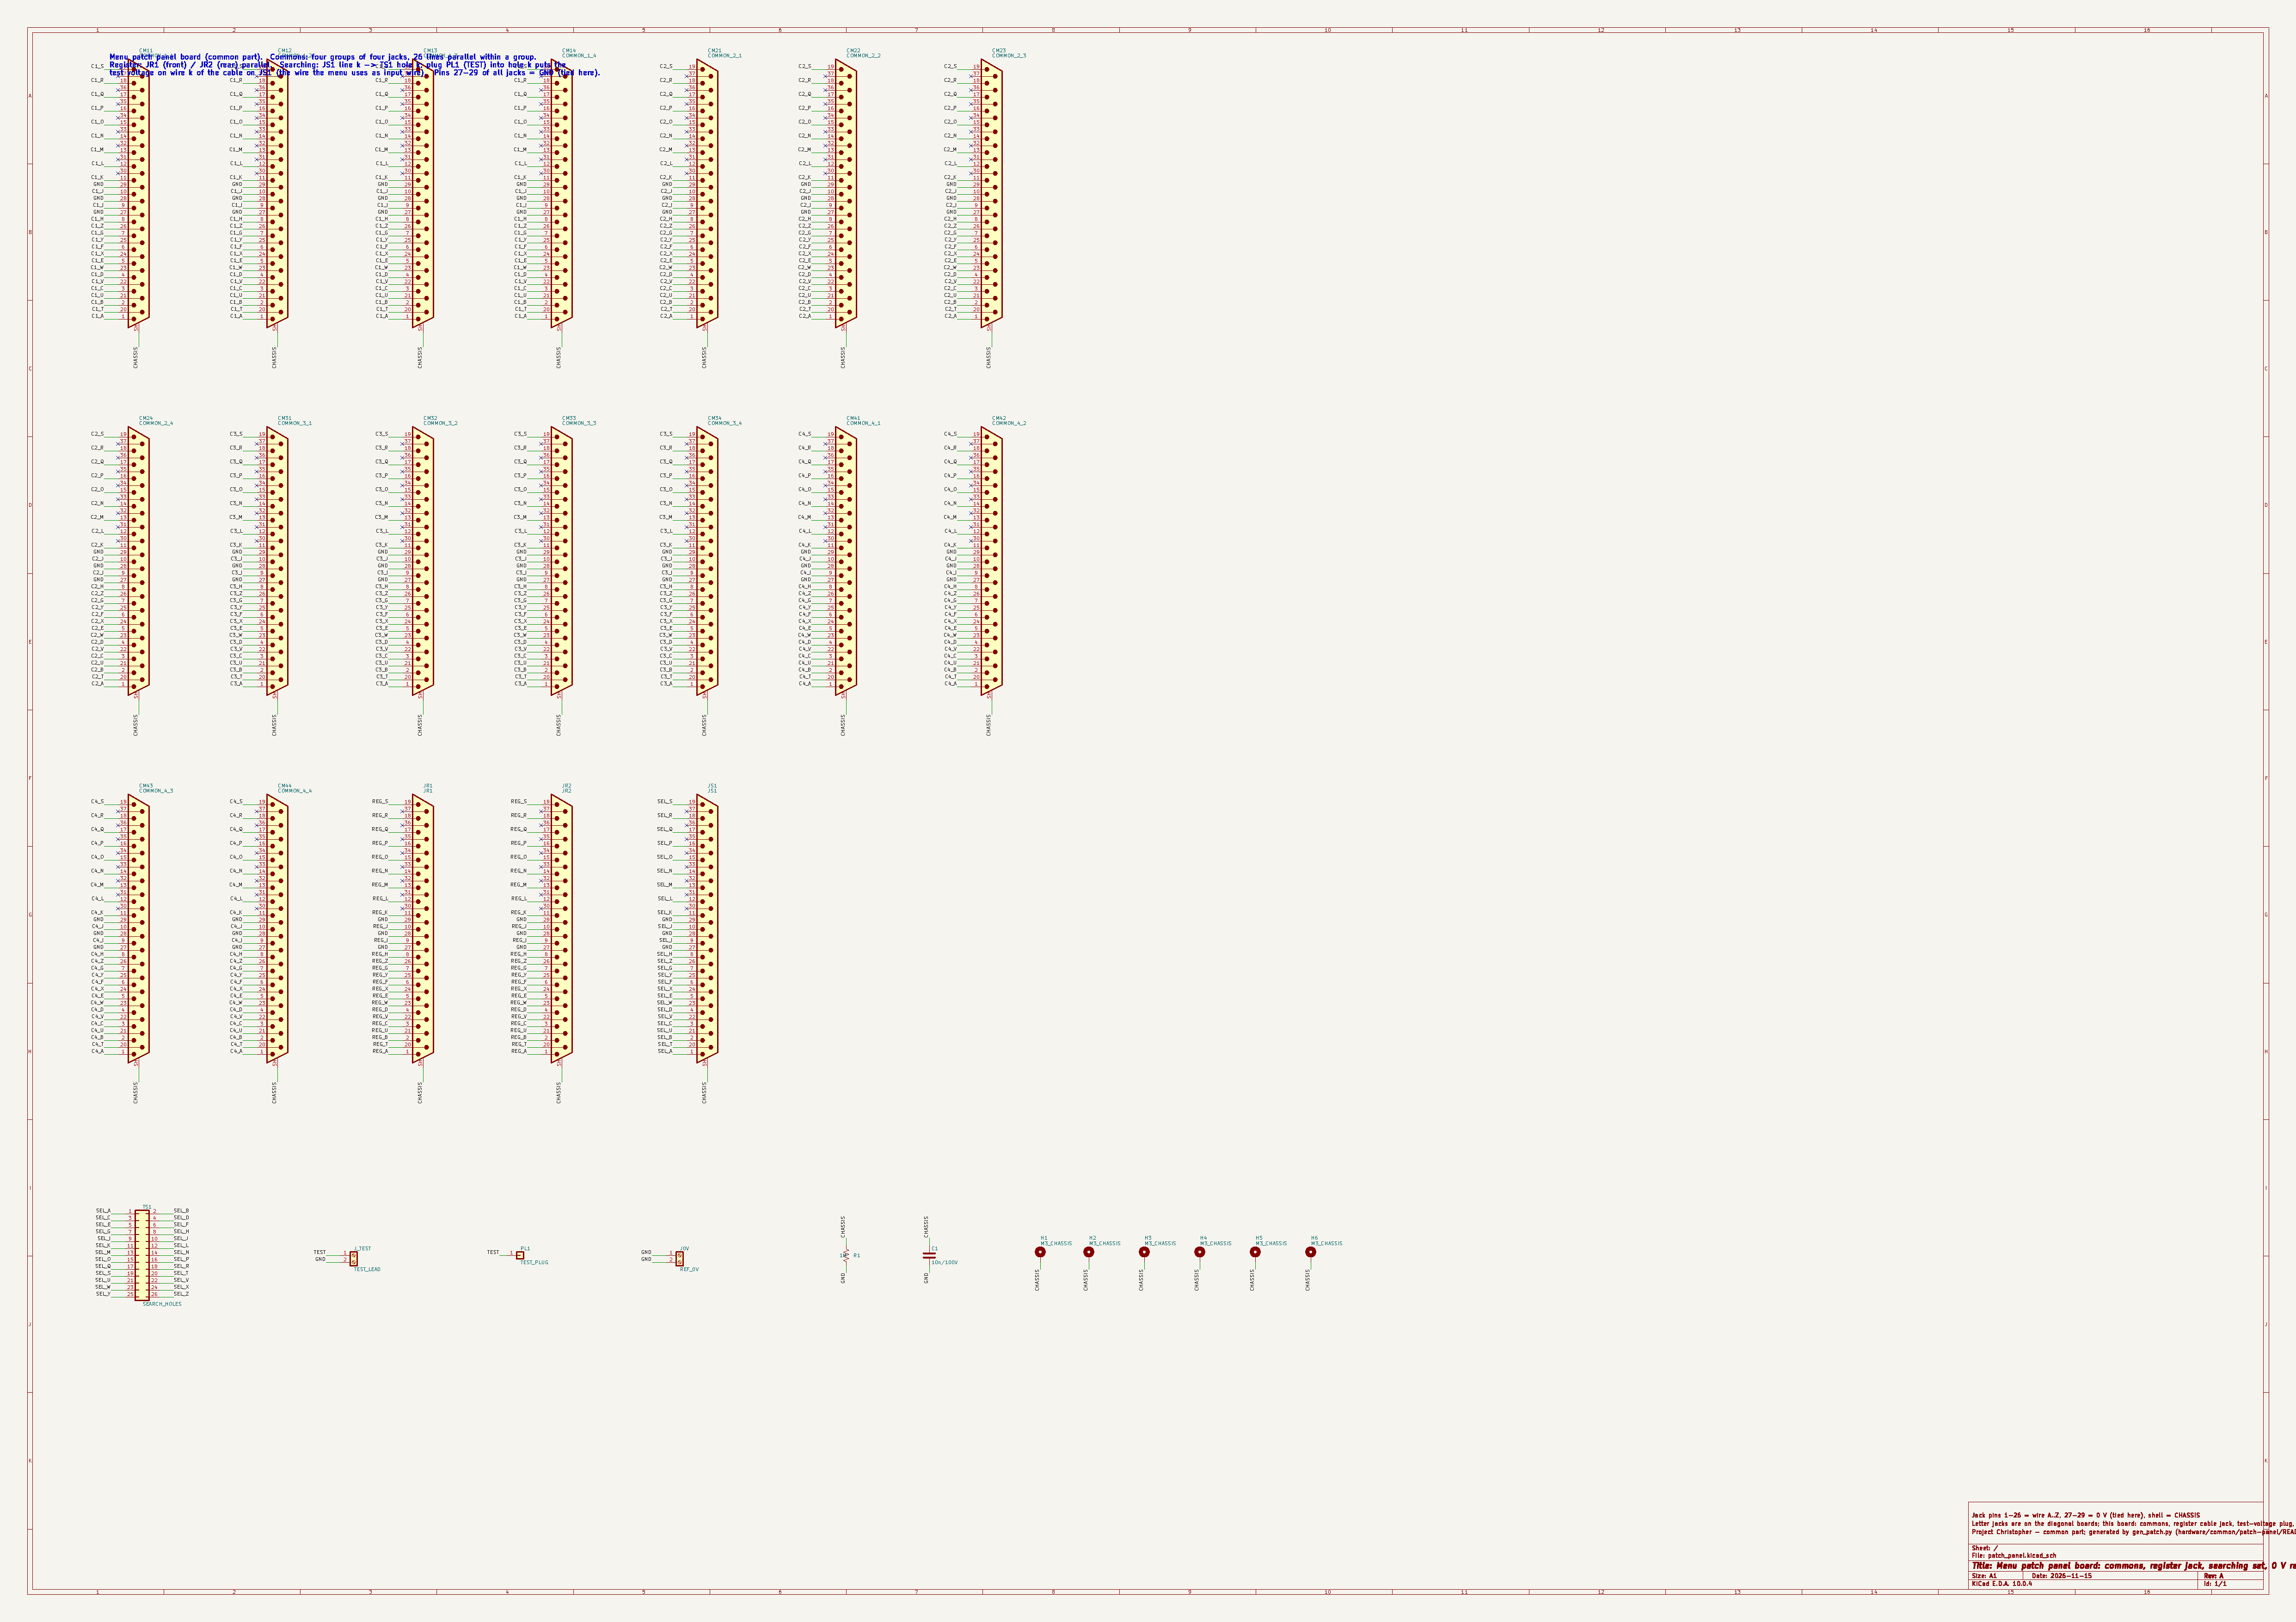
\includepdf[pages=-,pagecommand={\thispagestyle{plain}}]{figures/generated/sch_patch-panel.pdf}}{}
